\section{Inference using Linear Hybrid Models}
In this section we generalise the graphical models of the previous sections as shown in Figure \ref{fig_hybridmod1}. We include the discrete random variables, $s_1, s_2,...$ where each variable has $N$ states, which we will call the switching variables. The goal of adding switching variables is to allow our graphical models to switch (or more precisely, choose based on the observation) between $N$ different dynamical models. For the moment we restrict ourselves to linear transition functions i.e. we use linear state space models. The other variables retain their meaning as before. Models of this form are usually called Switching Kalman Filter models \cite{murphy1}. 
\begin{figure}[H] 
\centering
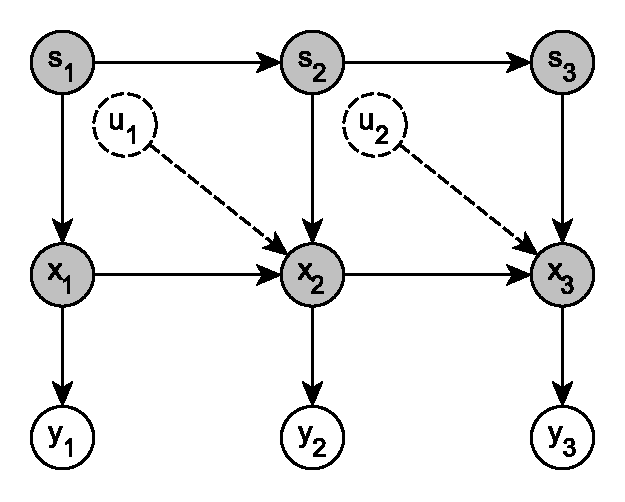
\includegraphics[scale=1.0]{hybrid_model.pdf}
\caption{Graphical model of this section}
\label{fig_hybridmod1}
\end{figure}
One of the benefits of combining discrete switching variables with linear dynamical models is that it allows us to model nonlinear processes with linear models. Intuitively, we can glue together linear models which each describe a nonlinear model in some region and use the switch to determine which one to use. The switch assigns a weight to each model based on its ability to explain the evidence. 

We model this system as follows. Let $s_t \in (1,2,..., N)$ denote a discrete, time homogeneous $N$ state first order Markov chain with transition matrix $P$ as discussed in the Hidden Markov Model section. Let each state $s_t=i$ be associated with a parameter set $\left(A_i, B_i, b_i, Q_i, C_i, R_i \right)$ used to evaluate the dynamical model shown in (\ref{eq_smodel}). If $s_t$ were observed then (\ref{eq_smodel}) would simplify to a set of linear latent dynamical systems we could perform inference on using the methods investigated in the Linear Models section. However, we assume that $s_t$ is a hidden random variable.
\begin{equation}
\begin{aligned}
x_{t+1} &= A_ix_t + B_iu_t + w_{t+1} \text{ with } \mathcal{N}(w_{t+1}|0,W_i) \\
y_{t+1} &= C_ix_{t+1} + v_{t+1}  \text{ with } \mathcal{N}(v_{t+1}|0,V_i)
\end{aligned}
\label{eq_smodel}
\end{equation}
To fully specify the system we also require the prior distributions $p(s_1)$ and $p(x_1|s_1)$ as well as the transition matrix $P$. For the purposes of this dissertation we calculate the transition matrix based on the Euclidean distance between the linearisation points of the linear models. Suppose there are $N$ linear models. The transition from the model to itself is $\frac{N}{\sum_{i=1}^N i}$. The transition from the model to the next closest model is $\frac{N-1}{\sum_{i=1}^N i}$. Continuing in this way we can construct the stochastic matrix $P$.

\subsection{Exact Filtering}
The switching variables ($s_1, s_2,...$) are discrete random variables exactly like the ones seen in the Hidden Markov Model section. There we derived recursive analytic expressions for inference which were computationally inexpensive. The stochastic linear dynamical system ($x_1,x_2,...$ and $y_1, y_2,...$) is exactly the same as the section on Linear Models. There we derived the famous Kalman Filter equations which were also analytic, recursive and computationally inexpensive. Taking this into consideration it seems plausible to believe that inference, specifically filtering, for hybrid systems like (\ref{eq_smodel}) can be formulated in a computationally feasible manner. 

Unfortunately, it can be shown that this is not possible in general \cite{lerner}\cite{murphy3} because the memory requirements scale exponentially with time. Loosely speaking one can see this by noting that at the first time step the system is described by a weighted set of $N$ Kalman Filter models (due to the linear assumption and the $N$ switching indices). At time step two the system is described by a weighted set of $N^2$ Kalman Filter models. Continuing in this manner we see that at time step $t$ the memory requirement is $N^t$. Clearly this is computationally infeasible and calls for approximate methods to be used. 

In literature many approximate filtering algorithms exist and it is not clear which is best. Two of the more popular methods include Gaussian Sum Filtering \cite{barber2} and Particle Filtering based methods (specifically the Rao-Blackwellisation approach, see \cite{chen}\cite{doucet}). Both of these methods take advantage of the Gaussian structure of the system and operate in a fixed memory space making them computationally attractive. We focus on the Particle based methods because it can be extended to nonlinear systems with ease.   

\subsection{Rao-Blackwellised Particle Filter}
It is our objective to find the joint posterior distribution $p(s_{1:t}, x_{1:t}|y_{1:t})$. This joint posterior admits filtering of Figure \ref{fig_hybridmod1} if we discard the trajectory and focus only in $s_t,x_t$. By the chain rule we immediately have that $p(s_{1:t}, x_{1:t}|y_{1:t}) = p(s_{1:t}|y_{1:t})p(x_{1:t}|y_{1:t}, s_{1:t})$. Given $s_{1:t}$ we see that $p(x_{1:t}|y_{1:t}, s_{1:t})$ can be evaluated using the Kalman Filter equations and thus we are only concerned with finding some approximation for $p(s_{1:t}|y_{1:t})$. This is the essence of the Rao-Blackwellised Particle Filter - taking advantage of the Gaussian nature of the system to analytically evaluate a part of the posterior distribution \cite{doucet}.

Using the formulation of the adaptive Sequential Importance Sampling algorithm discussed in the previous section we can apply it to find an approximation of $p(s_{1:t}|y_{1:t})$. We set $\gamma_t(s_{1:t})=p(s_{1:t},y_{1:t})$ and $Z_t=p(y_{1:t})$ and then have that $\frac{\gamma_t(s_{1:t})}{Z_t} = p(s_{1:t}|y_{1:t})$ as desired. We then choose our proposal distribution $q_t(s_{1:t}|y_{1:t})$ to be recursive and follow the same procedure as before shown in (\ref{eq_rbweight1}).
\begin{equation}
\begin{aligned}
w_t(s_{1:t}) &= \frac{\gamma_t(s_{1:t},y_{1:t})}{q_t(s_{1:t}|y_{1:t})} \\
&= \frac{p(s_{1:t},y_{1:t})}{q_t(s_{1:t}|y_{1:t})} \\
&\propto \frac{p(s_{1:t}|y_{1:t})}{q_t(s_{1:t}|y_{1:t})} \\
&\propto \frac{p(y_t|s_t)p(s_t|s_{t-1})}{q_t(s_t|s_{1:t-1},y_{1:t})}\frac{p(s_{1:t-1}|y_{1:t-1})}{q_t(s_{1:t-1}|y_{1:t-1})} \\
&= \alpha_t(s_{1:t})w_{t-1}(s_{1:t-1})
\end{aligned}
\label{eq_rbweight1}
\end{equation}
As before, we are not interested in the whole trajectory of the switching variable because we only need to perform filtering. Thus our proposal distribution can be chosen to be the prior i.e. $q_t(s_t|s_{1:t-1},y_{1:t}) = p(s_t|s_{t-1})$. This is suboptimal but easy to sample from \cite{doucet}. The incremental weight then simplifies to $\alpha_t(s_{1:t}) = p(y_t|s_t)$. We can evaluate this distribution by marginalising out $x_t$ and using the properties of the Gaussian distributions as before (\ref{eq_rbweight2}).
\begin{equation}
\begin{aligned}
\alpha_t(s_{1:t}) &= p(y_t|s_t) \\
&= \int_{x_t} p(y_t|x_t,s_t)p(x_t|s_{1:t},y_{1:t-1}) \\
&= p(y_t|y_{1:t-1}, s_{1:t}) \\
&= \mathcal{N}\left(y_t | C_{s_t}A_{s_t}\mu_{t-1}, C_{s_t}\left(A_{s_t}\Sigma_{t-1}A_{s_t}^T+Q_{s_t} \right)C_{s_t} + R_{s_t} \right)
\end{aligned}
\label{eq_rbweight2}
\end{equation} 
Where $s_t$ is denotes a specific state of the switching variable \cite{murphy1}. Upon inspection we see that (\ref{eq_rbweight2}) is just the one step ahead prediction likelihood as discussed in the Linear Models section on prediction \cite{murphy1}. Note that we will still need to resample $s_t$ from $P$ periodically to prevent sample impoverishment. 

We now have an efficient particle approximation of $p(s_t|y_t)$. To find the filtered posterior distribution as desired we note that $p(s_t,x_t|y_{1:t}) = \sum_i w_t^i(S_t^i)\delta(S_t^i, s_t)p(x_t|y_{1:t}, S_t^i)$ where $S_t^i$ is the i$^{\text{th}}$ particle. Each particle thus consists of a weight, a switch sample and the sufficient statistics generated by the Kalman Filter for a Gaussian i.e. a mean and covariance. The complete algorithm is shown below.

\textbf{Rao-Blackwellised Particle Filter Algorithm}\\
For $t=1$:
\begin{enumerate}
\item
Sample $S^i_1 \backsim p(s_1)$ and $\mu_{1|0}^i \backsim p(x_1|s_1)$.
\item
Compute the weights $w_1(S_1^i) = p(Y^*_1|S_1^i)$ where $Y^*_1$ is the observation. Normalise $W^i_1 \propto w_1(S^i_1)$.
\item
Apply the update step of the Kalman Filter to each particle $i$ and associated parameters to find $\mu_1^i$ and $\Sigma_1^i$. 
\item
If the number of effective particles is below some threshold apply resampling with roughening $(W^i_1, {S}^i_1,{\mu}^i_1, {\Sigma}^i_1)$ to obtain $N$ equally weighted particles $(\frac{1}{N}, \bar{S}^i_1, \bar{\mu}^i_1, \bar{\Sigma}^i_1)$ and set $(\bar{W}^i_1, \bar{S}^i_1, \bar{\mu}^i_1, \bar{\Sigma}^i_1) \leftarrow (\frac{1}{N}, \bar{S}^i_1, \bar{\mu}^i_1, \bar{\Sigma}^i_1)$ otherwise set $(\bar{W}^i_1, \bar{S}^i_1, \bar{\mu}^i_1, \bar{\Sigma}^i_1) \leftarrow ({W}^i_1, {S}^i_1, \mu^i_1, \Sigma_1^i)$
\end{enumerate}
For $t \geq 2$:
\begin{enumerate}
\item
Sample $S^i_t \backsim p(S_t^i|\bar{S}^i_{t-1})$.
\item
Compute the weights $\alpha_t(S^i_{t}) = p(Y^*_t|S_t^i)$ and normalise $W^i_t \propto \bar{W}^i_{t-1}\alpha_t(S^i_{t})$.
\item
Apply the Kalman Filter algorithm to $\mu_{t-1}$ and $\Sigma_{t-1}$ for each particle $i$ to find the sufficient statistics $\mu_{t}$ and $\Sigma_{t}$ using the parameters corresponding to the state of $S^i_t$.
\item
If the number of effective particles is below some threshold apply resampling with roughening $(W^i_t, {S}^i_t,{\mu}^i_t, {\Sigma}^i_t)$ to obtain $N$ equally weighted particles $(\frac{1}{N}, \bar{S}^i_t, \bar{\mu}^i_t, \bar{\Sigma}^i_t)$ and set $(\bar{W}^i_t, \bar{S}^i_t, \bar{\mu}^i_t, \bar{\Sigma}^i_t) \leftarrow (\frac{1}{N}, \bar{S}^i_t, \bar{\mu}^i_t, \bar{\Sigma}^i_t)$ otherwise set $(\bar{W}^i_t, \bar{S}^i_t, \bar{\mu}^i_t, \bar{\Sigma}^i_t) \leftarrow ({W}^i_t, {S}^i_t, \mu^i_t, \Sigma_1^t)$
\end{enumerate} 

\subsection{Rao-Blackwellised Particle Prediction}
Like the Particle Predictor studied in the previous section, performing prediction using Rao-Blackwellisation is straightforward because there is no weighting (updating the particles based on the observation) step. Each particle's switching state is merely propagated forward using the proposal distribution (the transition matrix $P$) and the Kalman prediction algorithm is used to evaluate the predicted mean and covariance. For the sake of brevity we do not supply an algorithm because it is a straightforward simplification of the Rao-Blackwellised Particle Filter Algorithm as shown above.

\subsection{Smoothing and Viterbi Decoding}
It is also possible to take advantage of the Gaussian structure in Figure \ref{fig_hybridmod1} to derive a so-called Rao-Blackwellised Smoothing Algorithm. We do not include it here because it is not necessary for the aims of this dissertation. We refer the reader to the relevant literature \cite{chen}\cite{doucet}. 

Viterbi decoding is likewise not within the scope of this dissertation and as such we refer the reader to \cite{murphy1} for more information. Suffice to say, by increasing the complexity of Figure \ref{fig_hybridmod1} we increase the difficulty of inference in general.

\subsection{Filtering the CSTR}
We now apply the Rao-Blackwellised Particle Filter to the CSTR introduced earlier. We first perform filtering on the CSTR by only measuring temperature. Since we are using linear models we compare the performance of the Switching Kalman Filter to that of the standard Kalman Filter which only uses one linear model. We then extend our system to measure both temperature and concentration and perform the same comparisons.

We use the same parameters as before and 500 particles unless otherwise stated. We also assume that the measurement and plant noise covariance matrices ($V,W$) are the same across all the models. To illustrate how the Switching Kalman Filter works we initially only use 3 linear models to perform inference. Figures \ref{fig_3mod_ss} to \ref{fig_3mod_t} show how  the filter performs using three linear models corresponding to the nominal operating points for the CSTR. We only measure temperature for the moment.

Figure \ref{fig_3mod_ss} shows where the linearisation points are with respect to the state space evolution of the system. We expect the Switching Kalman Filter to switch to models in the vicinity of its current position in the state space.
\begin{figure}[H] 
\centering
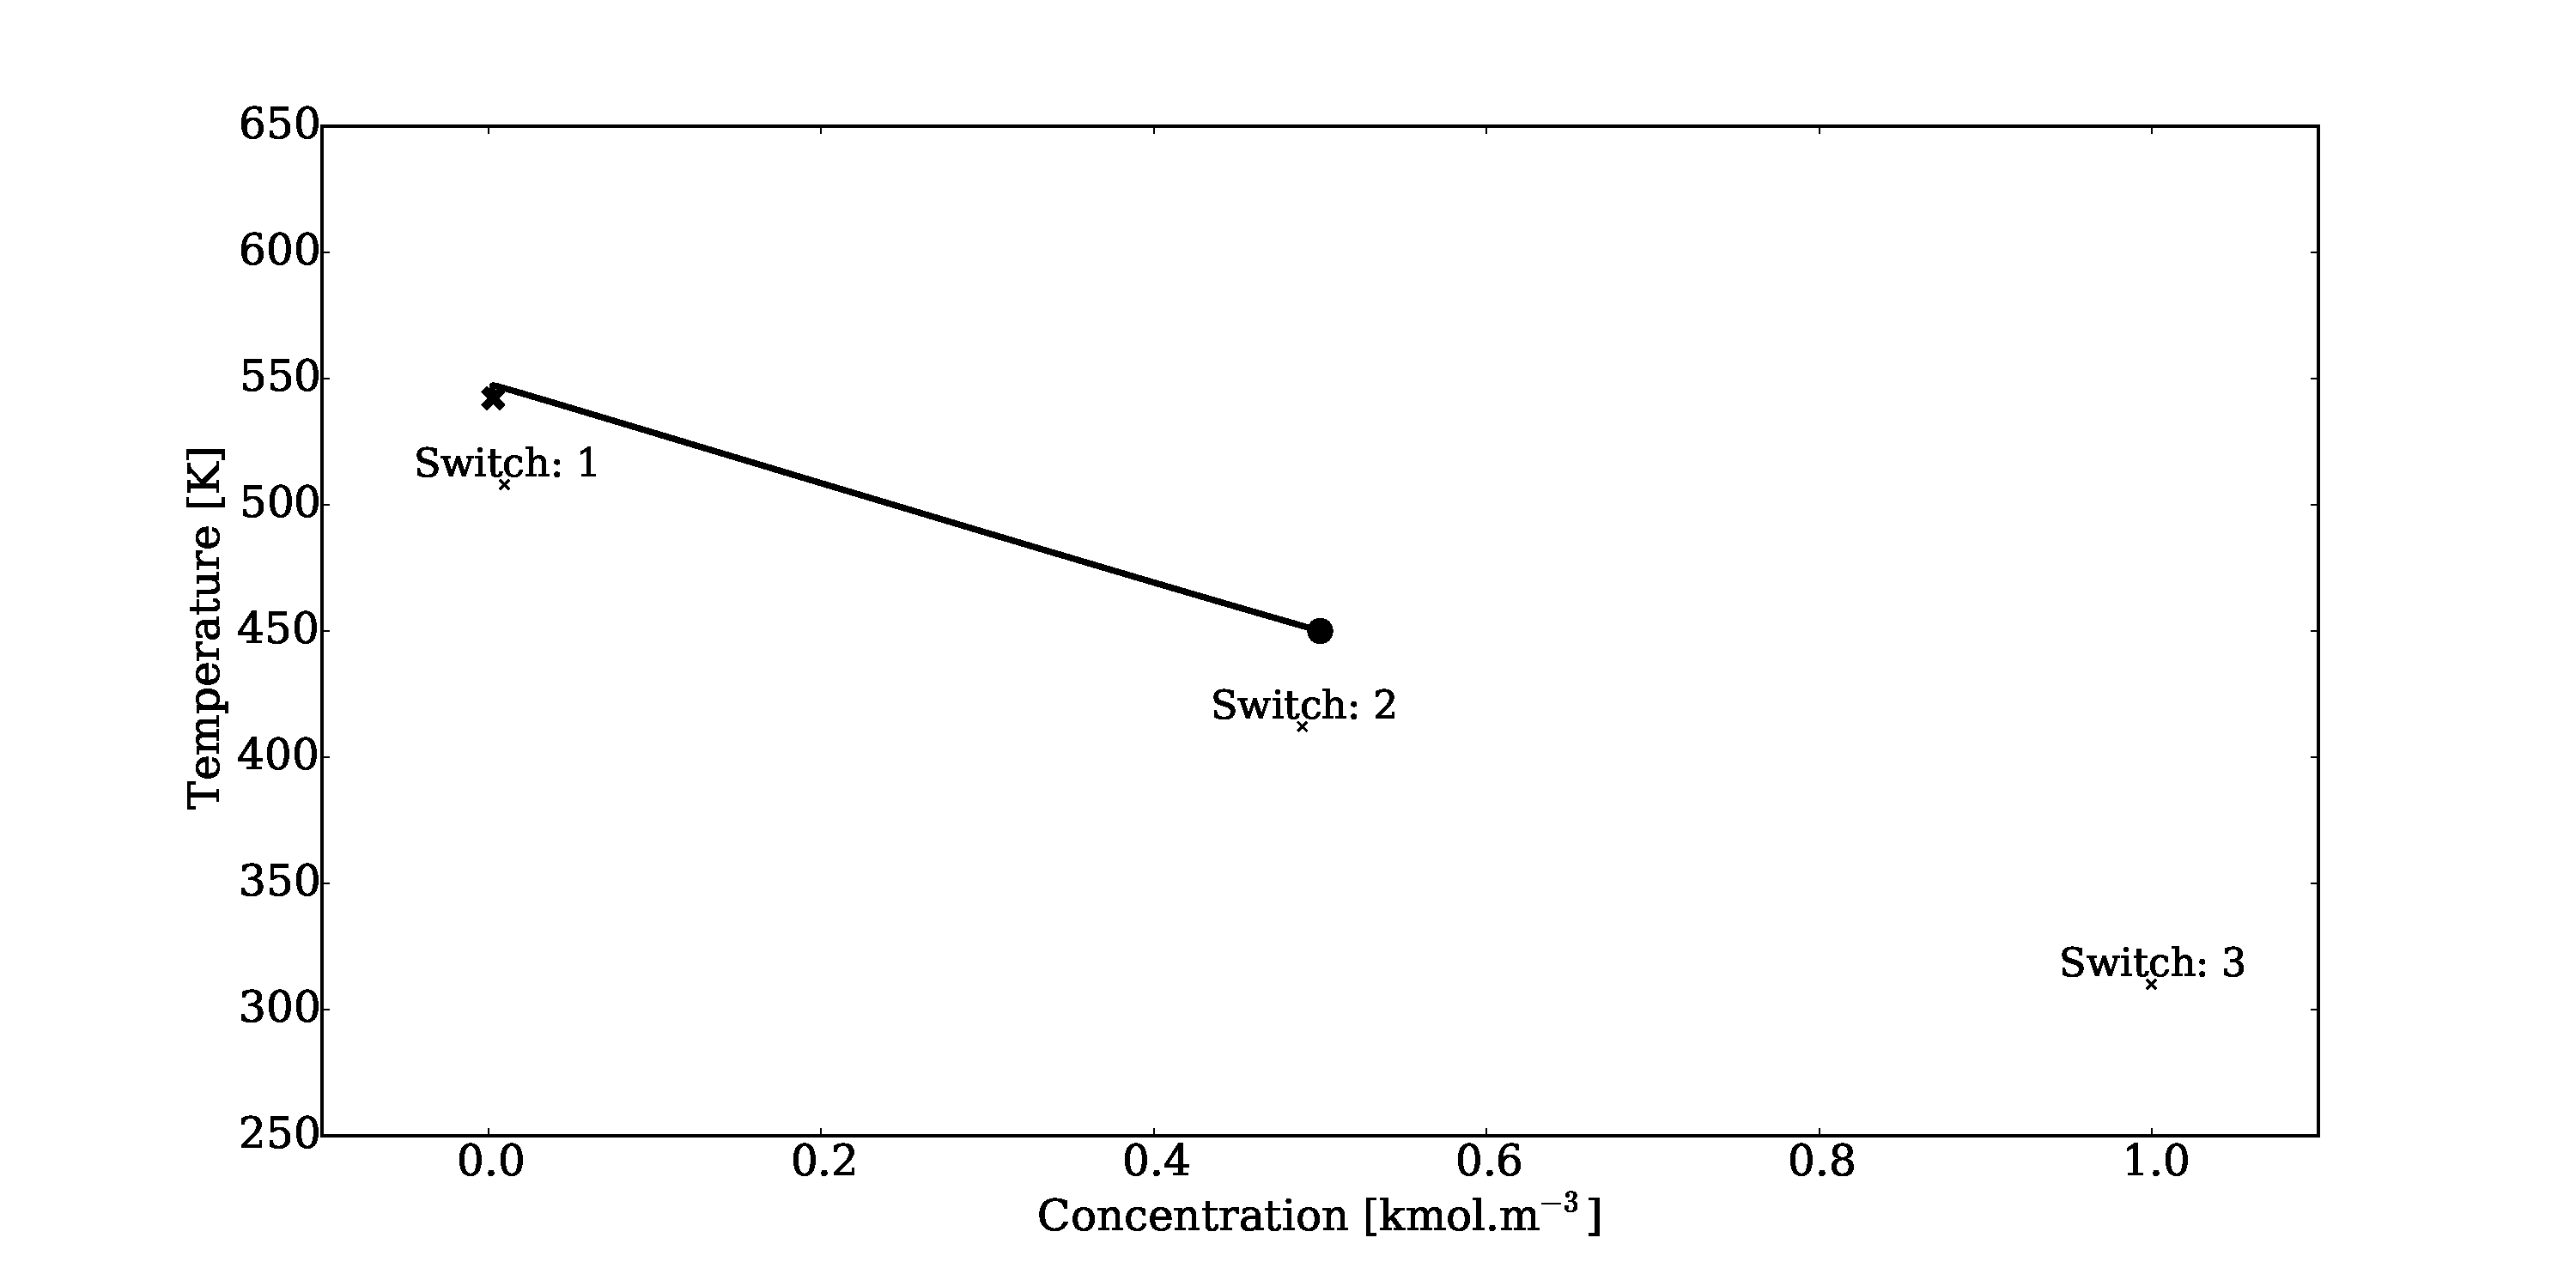
\includegraphics[scale=0.3]{skf_s3_s.pdf}
\caption{State space evolution and linearisation points of the three linear models used. The system starts at the black circle and ends at the black cross.}
\label{fig_3mod_ss}
\end{figure}
Figure \ref{fig_3mod_w} shows the weight of each model as time progresses. We see that the second model (S::2 aka switch 2) has the highest weight initially but after about 2 minutes the system switches models so that the first model (S::1 aka switch 1) has the highest weight. Intuitively the system has moved away from the region where the second model describes the system best into a region where the first model is a better descriptor. 
\begin{figure}[H] 
\centering
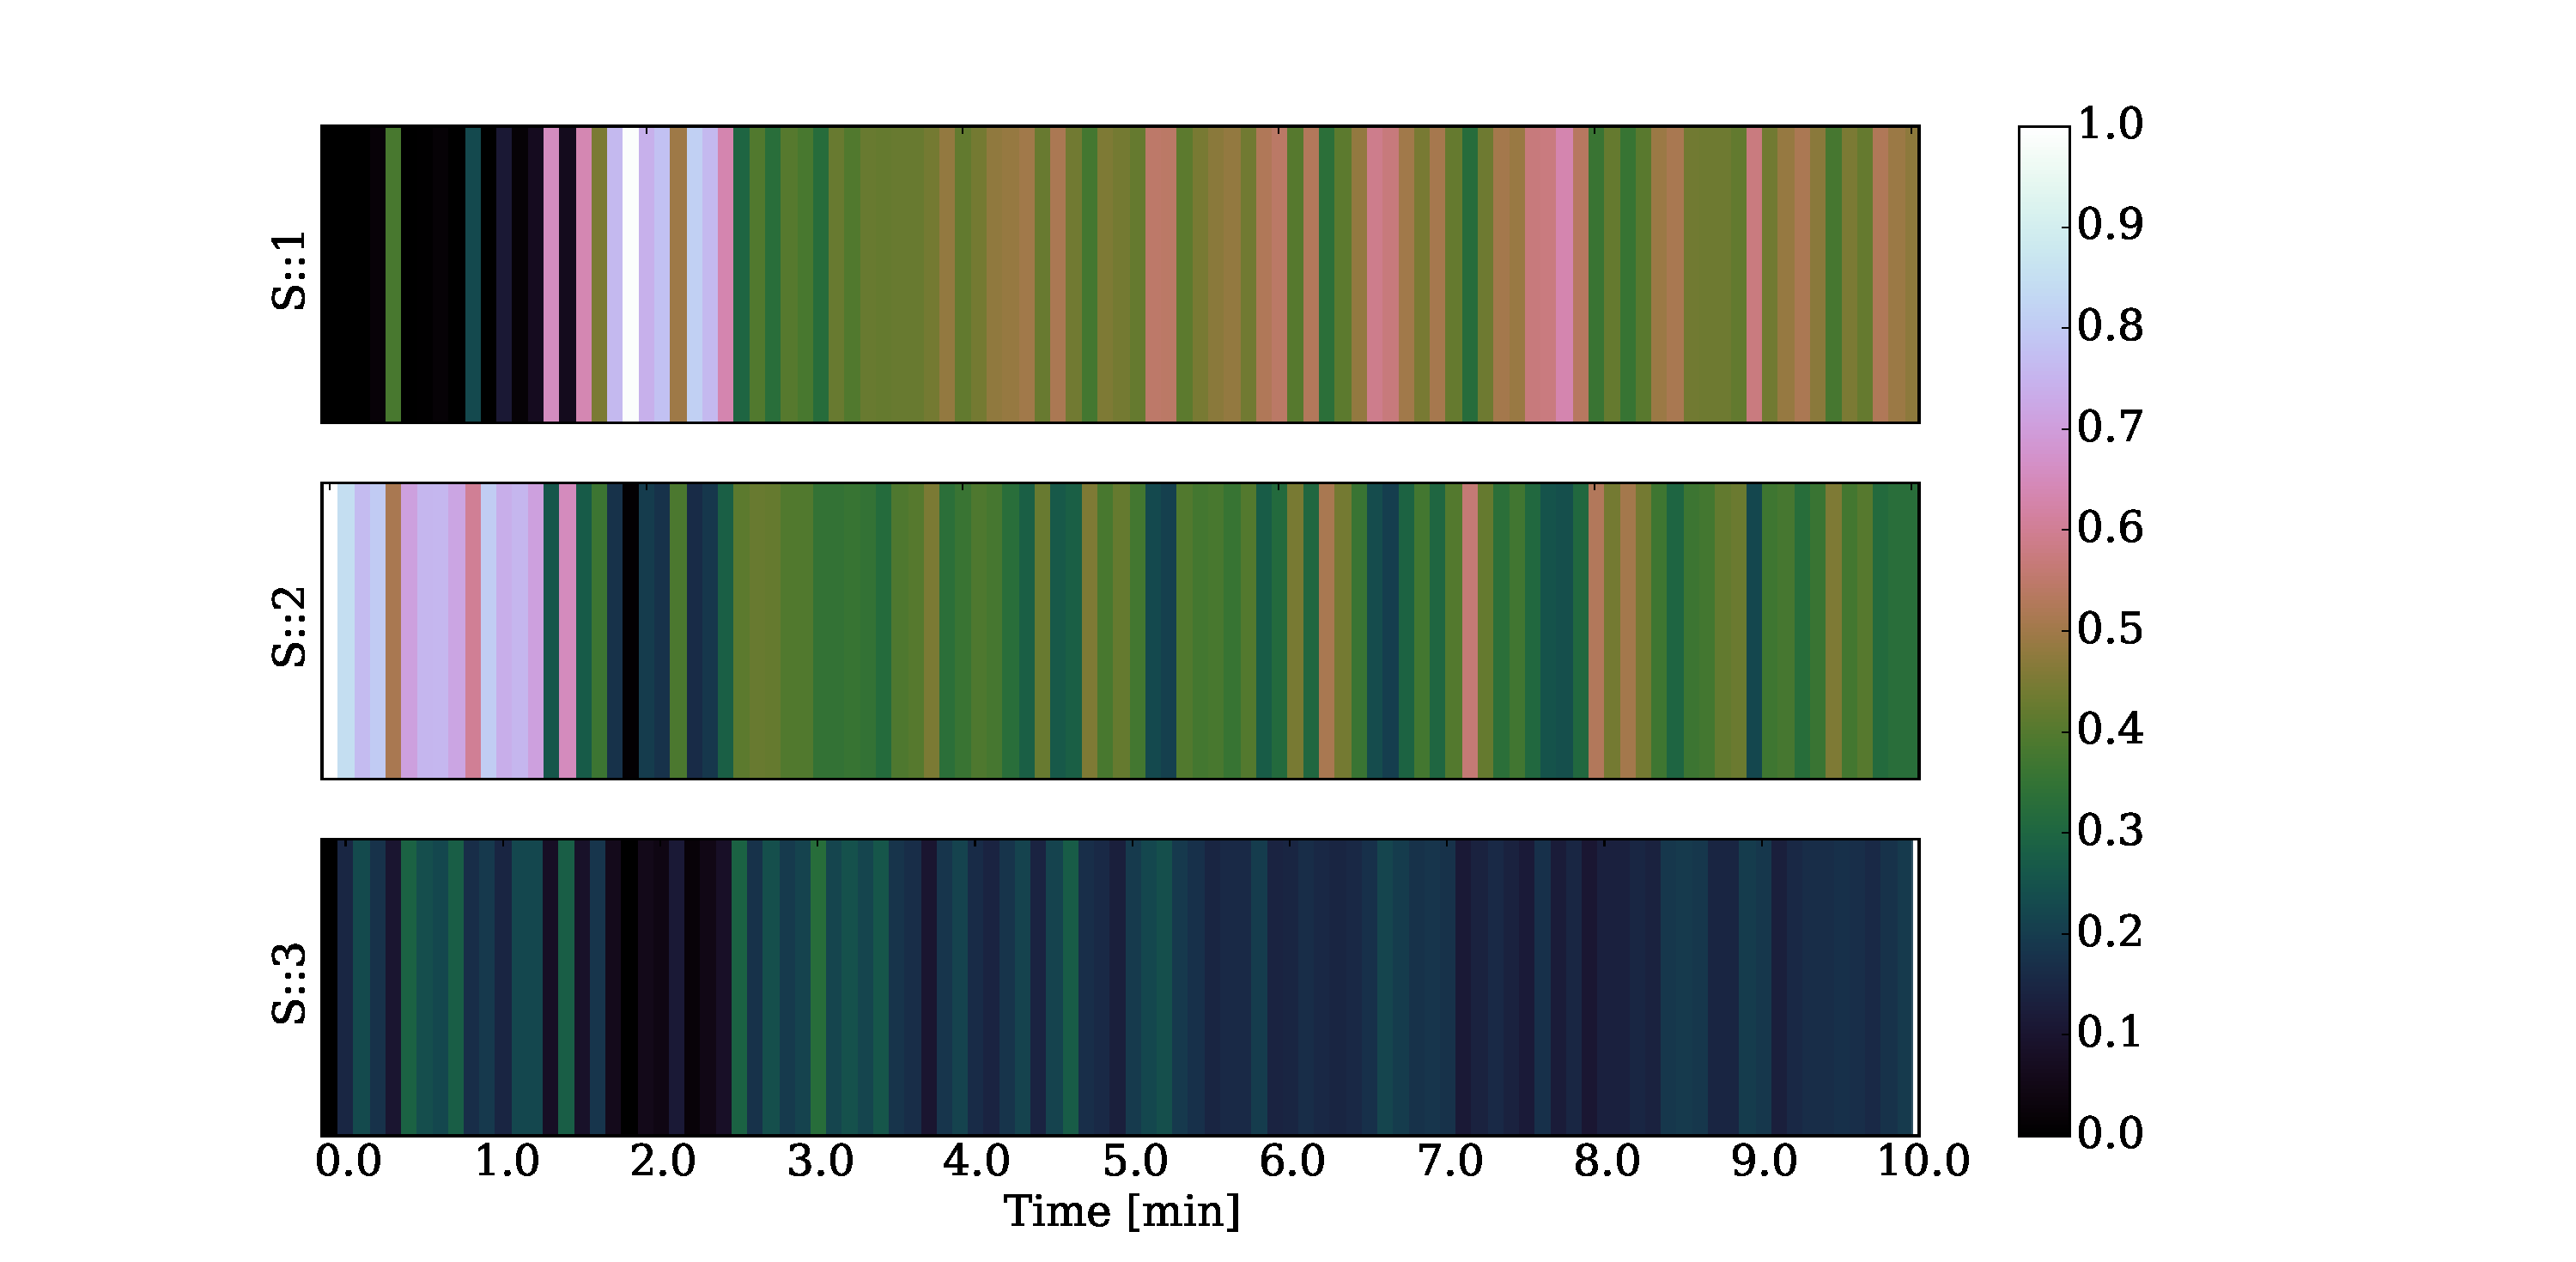
\includegraphics[scale=0.3]{skf_s3_w.pdf}
\caption{Weight of each switching index as time progresses.}
\label{fig_3mod_w}
\end{figure}
In Figure \ref{fig_3mod_t} we see the time series response of the system. Note that only temperature is measured but the system manages to track both states reasonably well. This is a vast improvement over the situation where only one linear model was used as in the section on Linear Models.
\begin{figure}[H] 
\centering
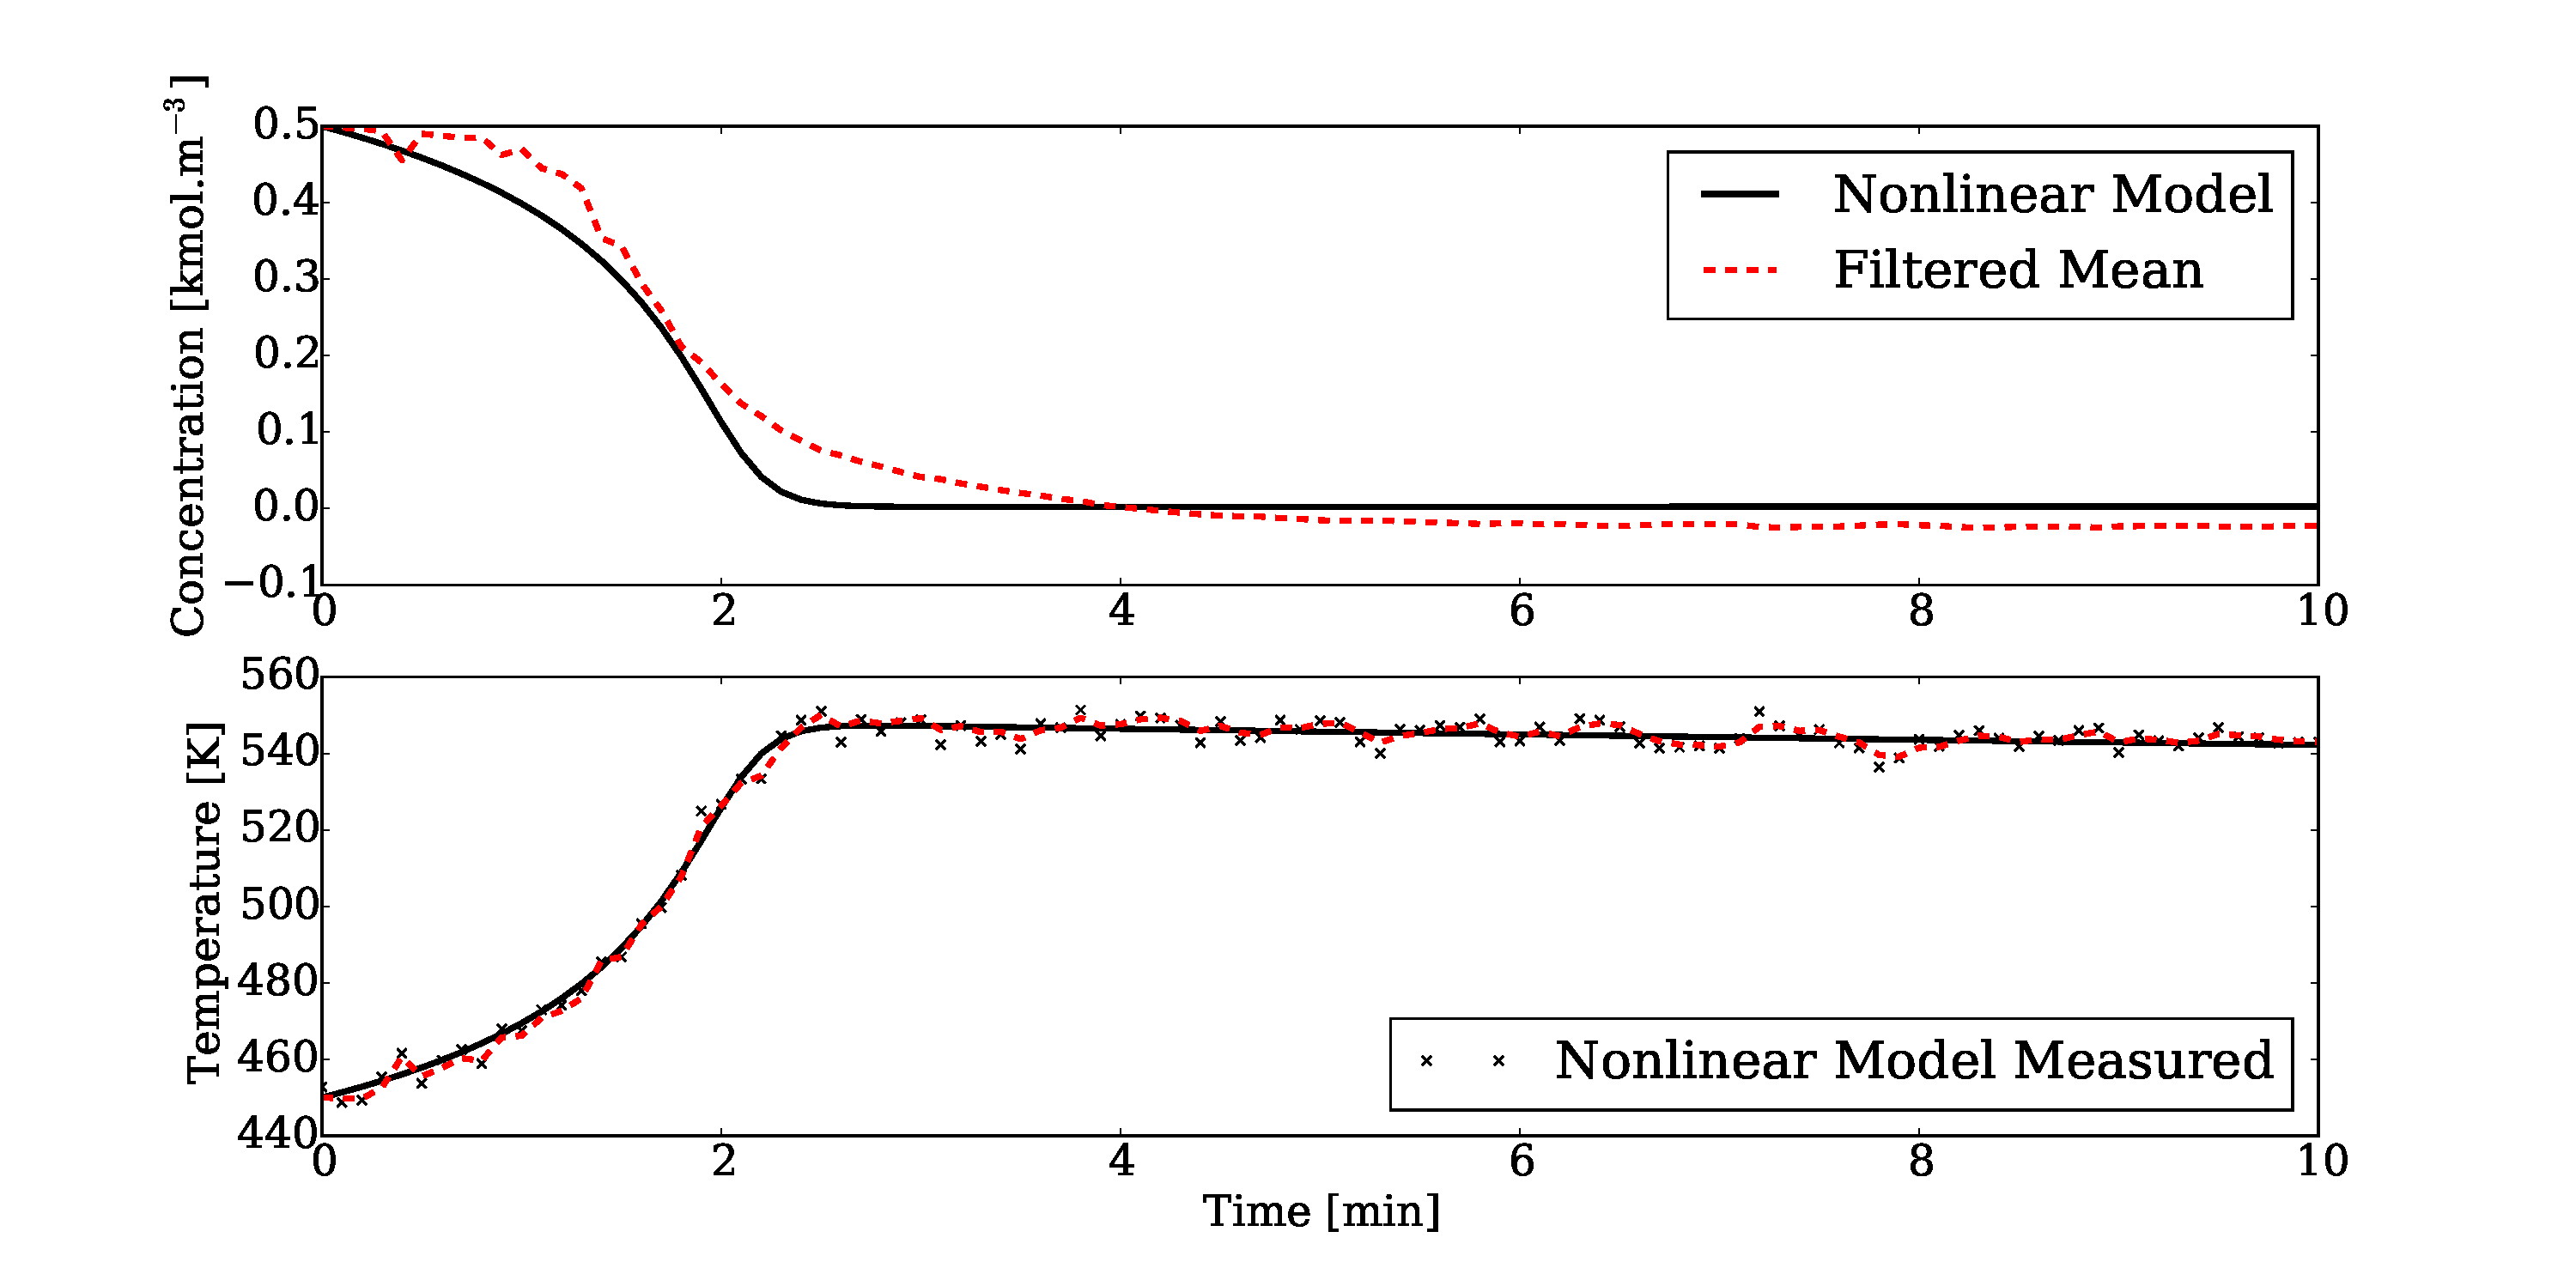
\includegraphics[scale=0.3]{skf_s3_t.pdf}
\caption{Time series evolution of the states with initial condition $(0.5, 450)$.}
\label{fig_3mod_t}
\end{figure}
Unfortunately, using only these three linear models is not adequate for this system. Since the models are far apart in the state space it sometimes happens that most of the particles are propagated forward using the wrong model. By not measuring a state this problem is exacerbated. Some of these incorrect models may predict the right temperature but the wrong concentration; consequently they are not weeded out by the weighting procedure because the concentration is not observed. The filter then fails to switch and this causes the filter to diverge from the true states. 

We illustrate this in Figures \ref{fig_3mod_s_w} to \ref{fig_3mod_t_w}. In Figure \ref{fig_3mod_s_w} we see the regions the CSTR traverses in the state space i.e. which switches we expect to be active. We expect switch 2 and 3 to be the most active.
\begin{figure}[H] 
\centering
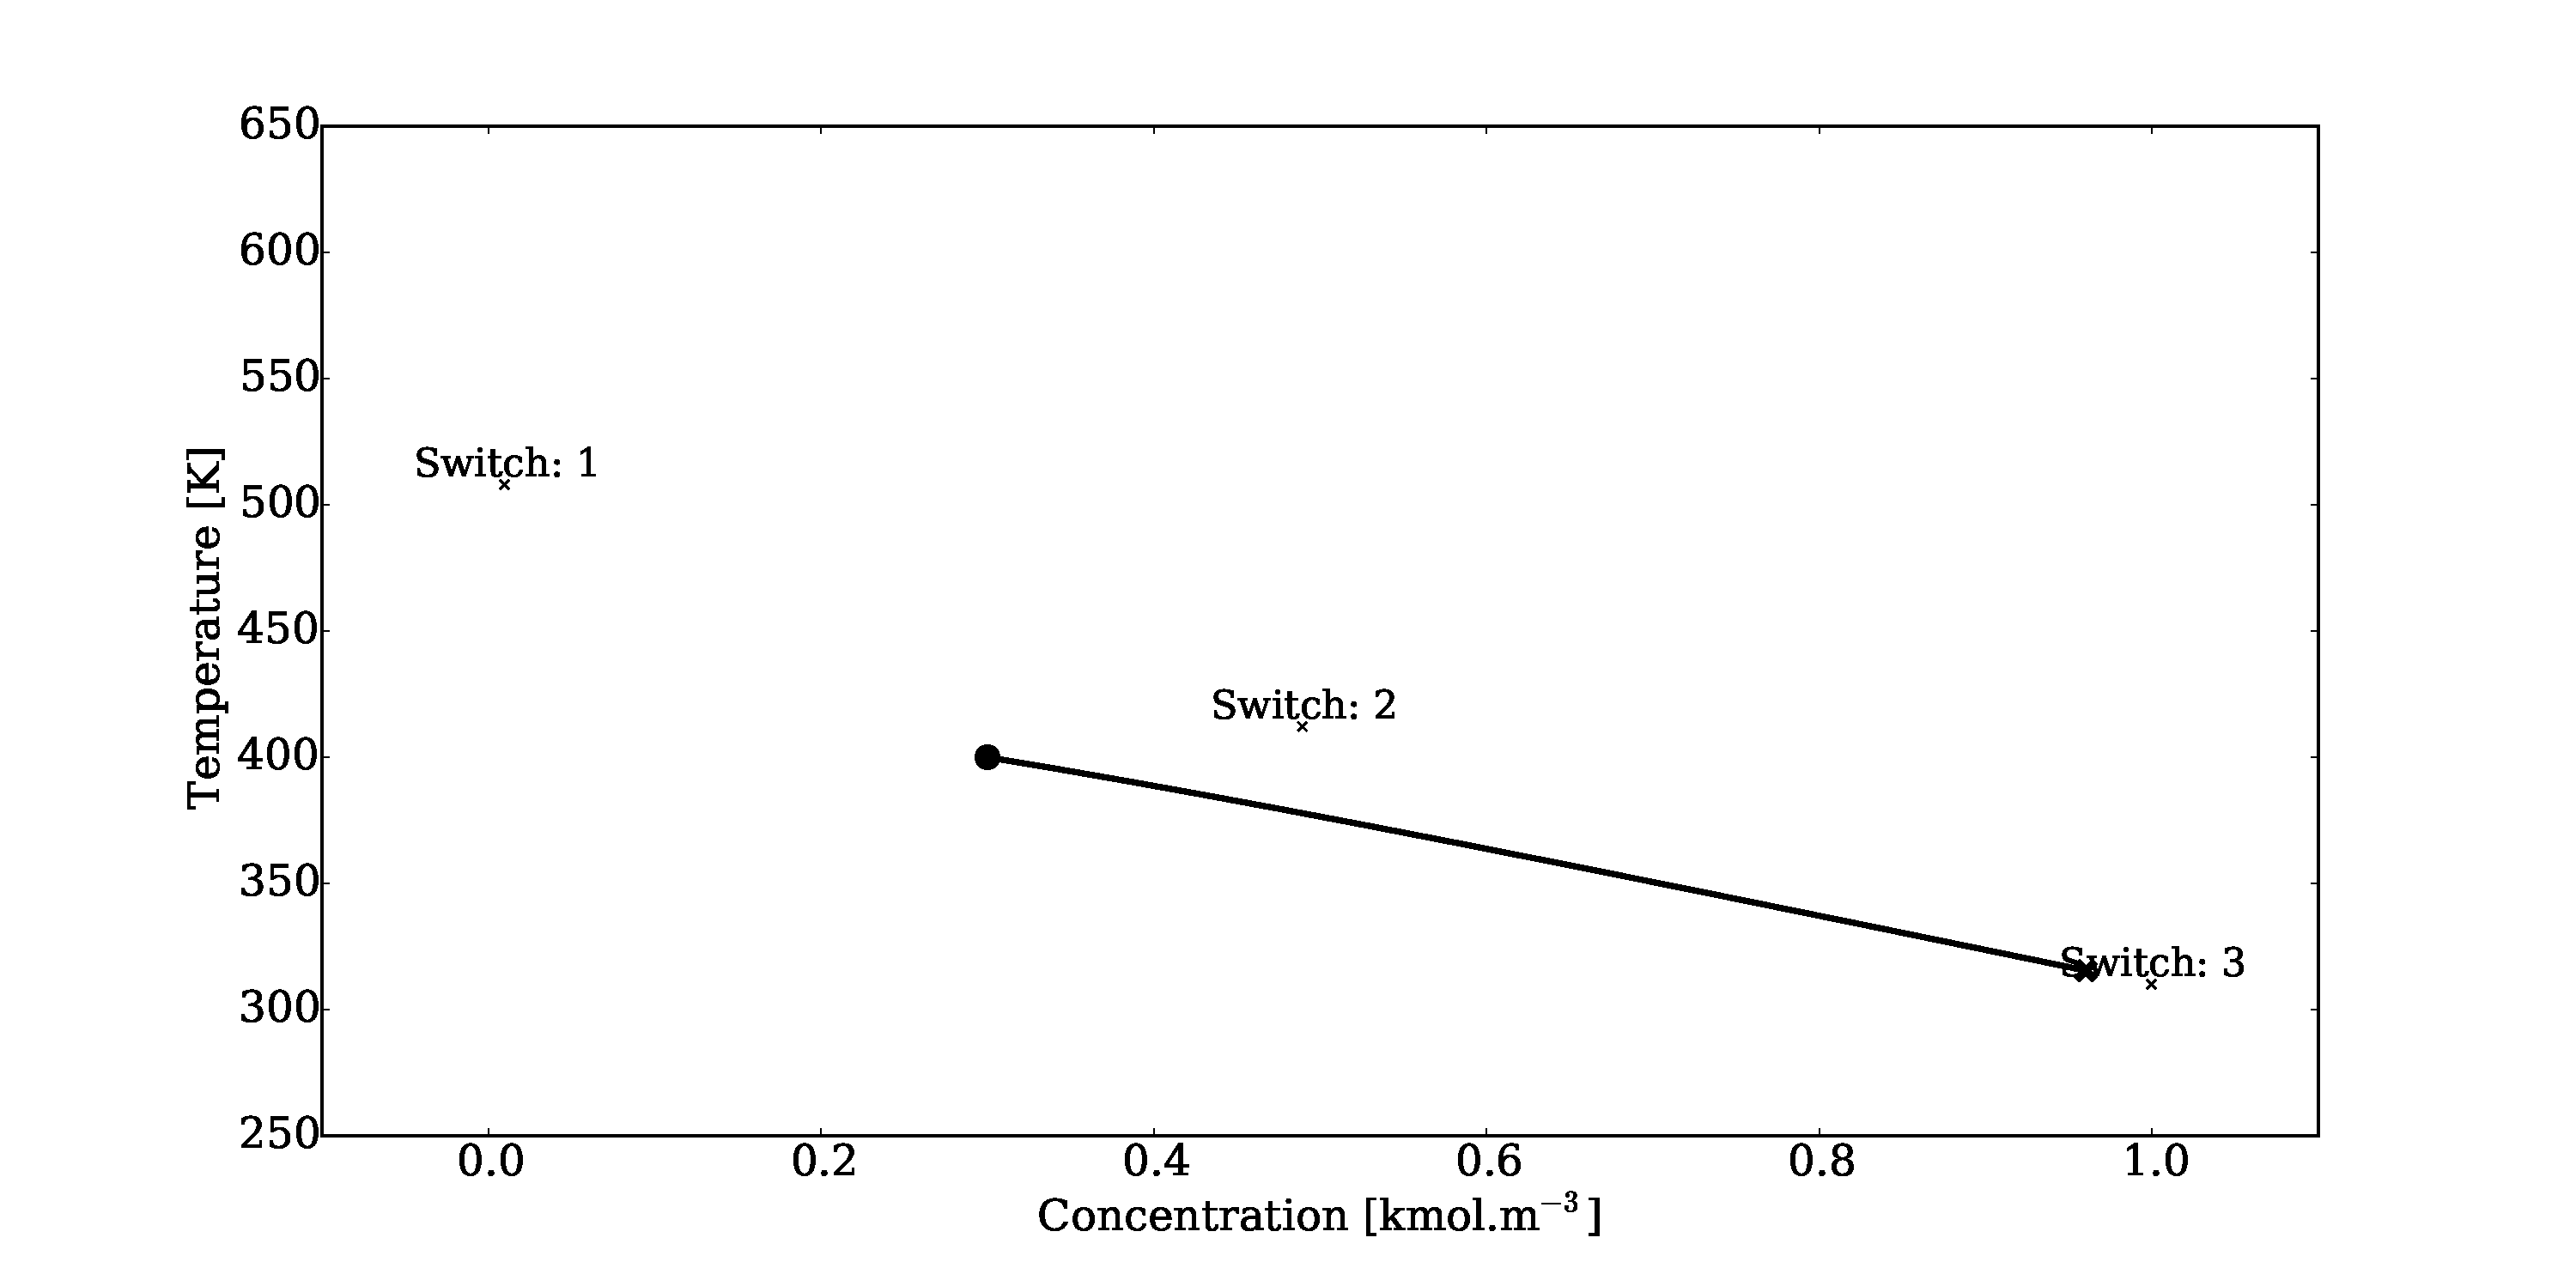
\includegraphics[scale=0.3]{skf_s3_s_w.pdf}
\caption{State space evolution and linearisation points of the three linear models used. The system starts at the black circle and ends at the black cross.}
\label{fig_3mod_s_w}
\end{figure}
Contrary to Figure \ref{fig_3mod_s_w} we see in Figure \ref{fig_3mod_w_w} that switch 1 and 2 are the most active. This causes filter divergence as seen in Figure \ref{fig_3mod_t_w}.
\begin{figure}[H] 
\centering
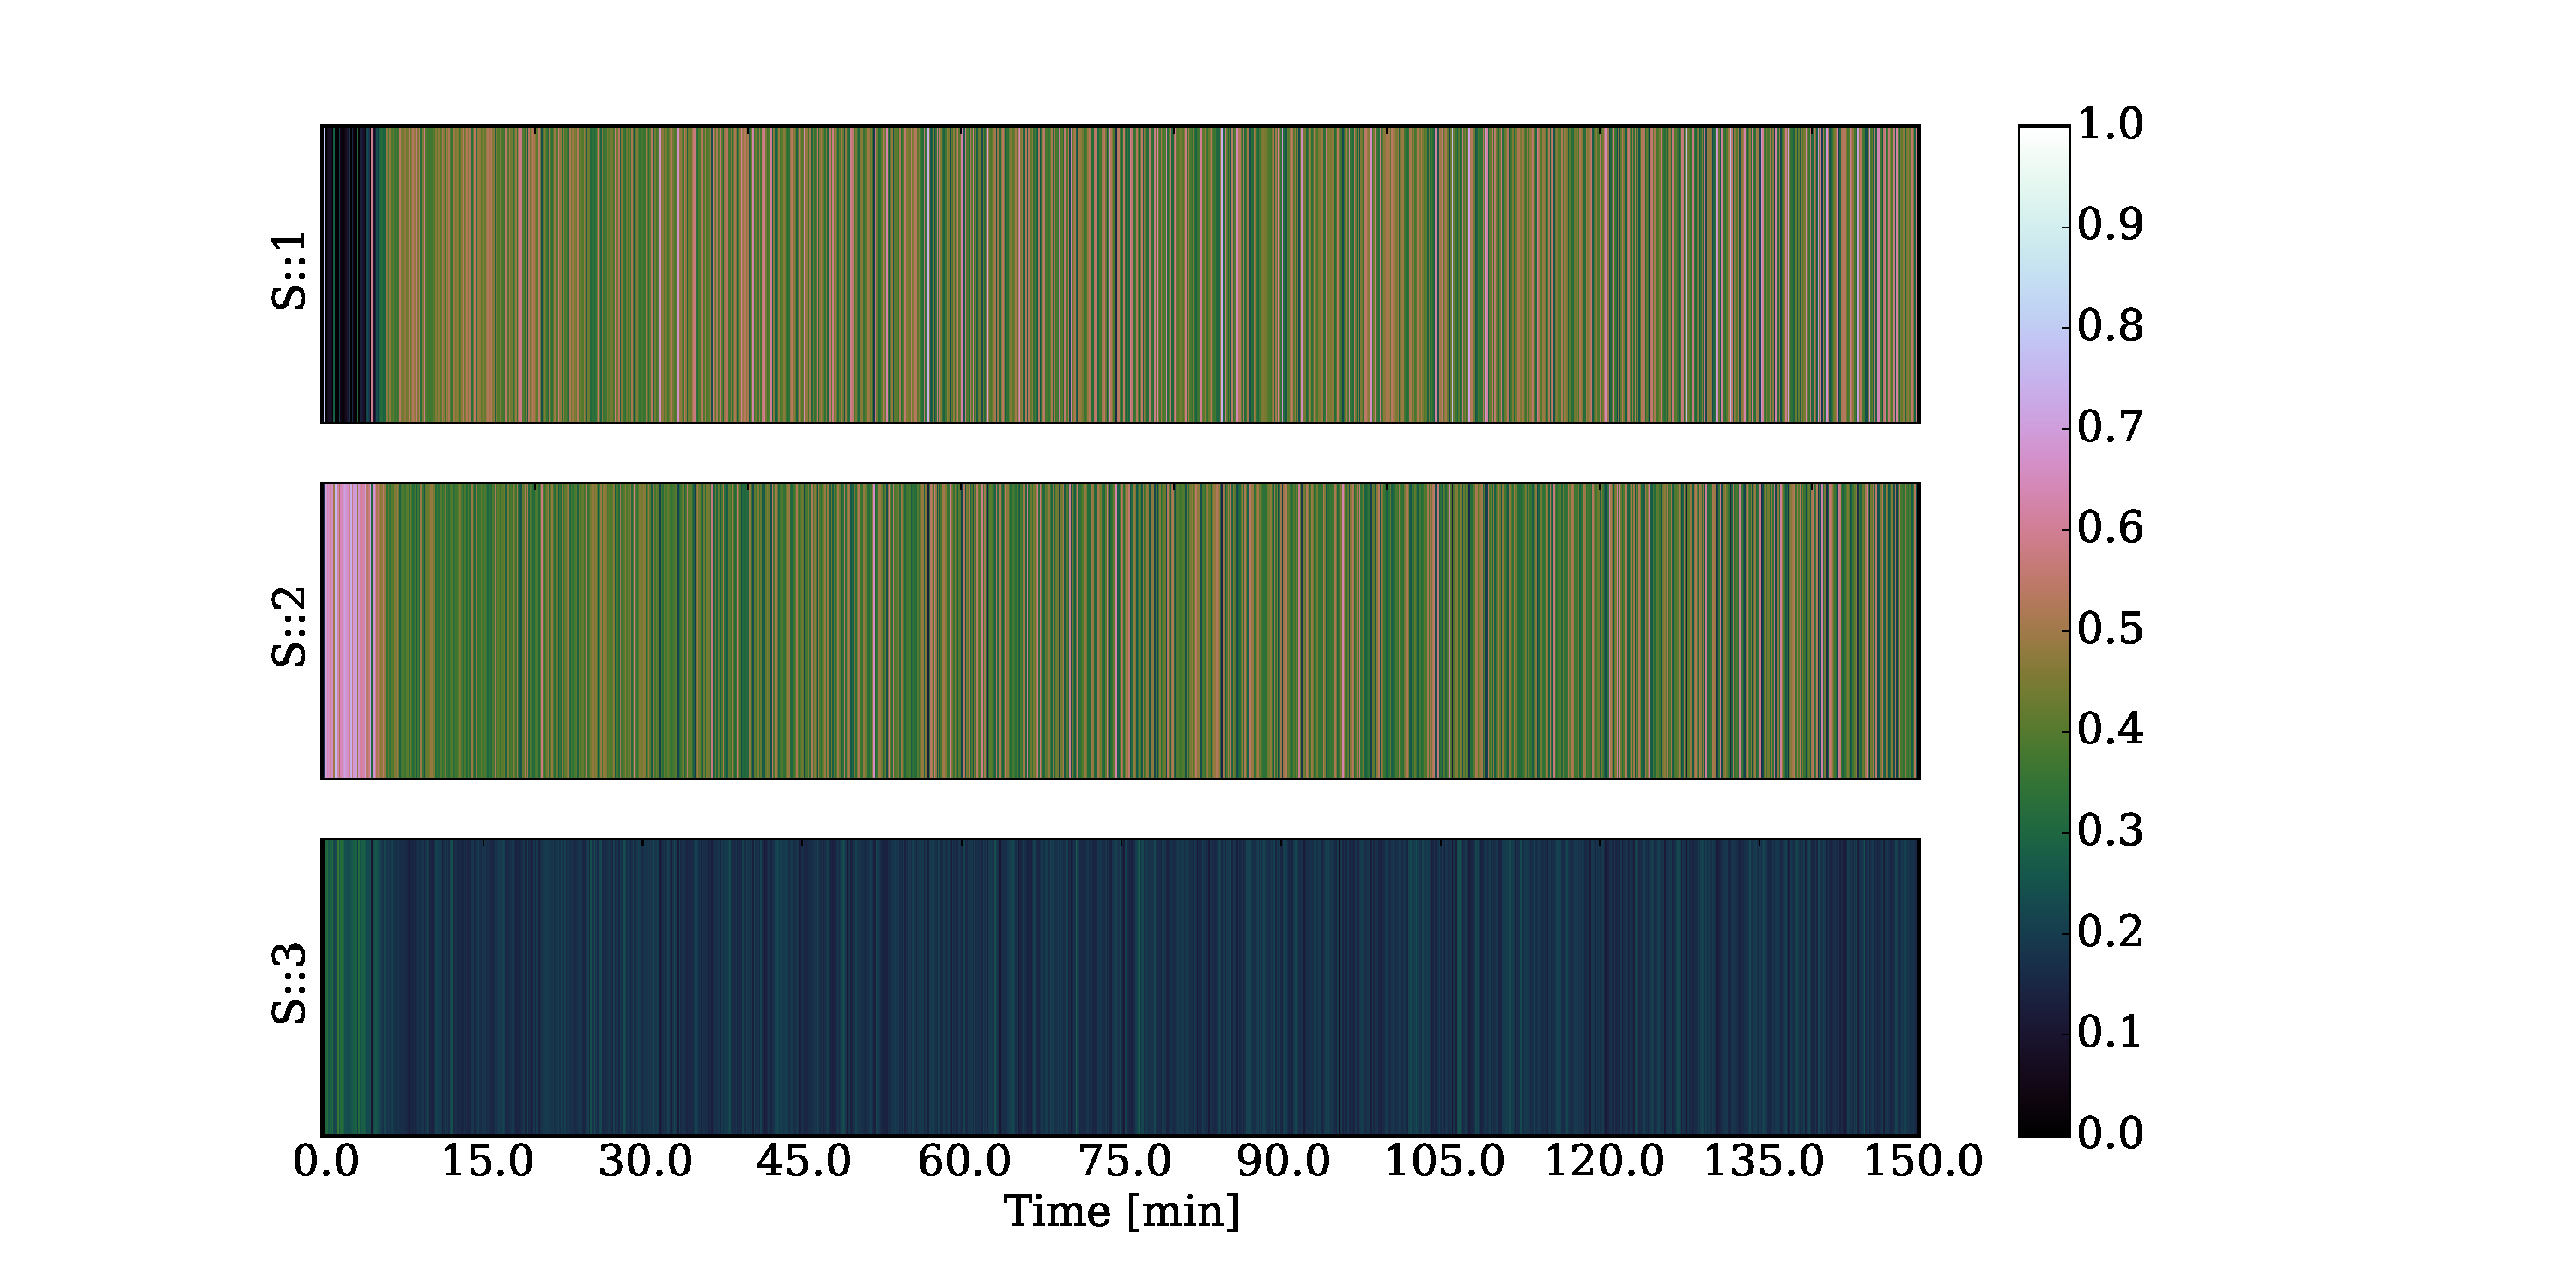
\includegraphics[scale=0.3]{skf_s3_w_w.pdf}
\caption{Weight of each switching index as time progresses.}
\label{fig_3mod_w_w}
\end{figure}
\begin{figure}[H] 
\centering
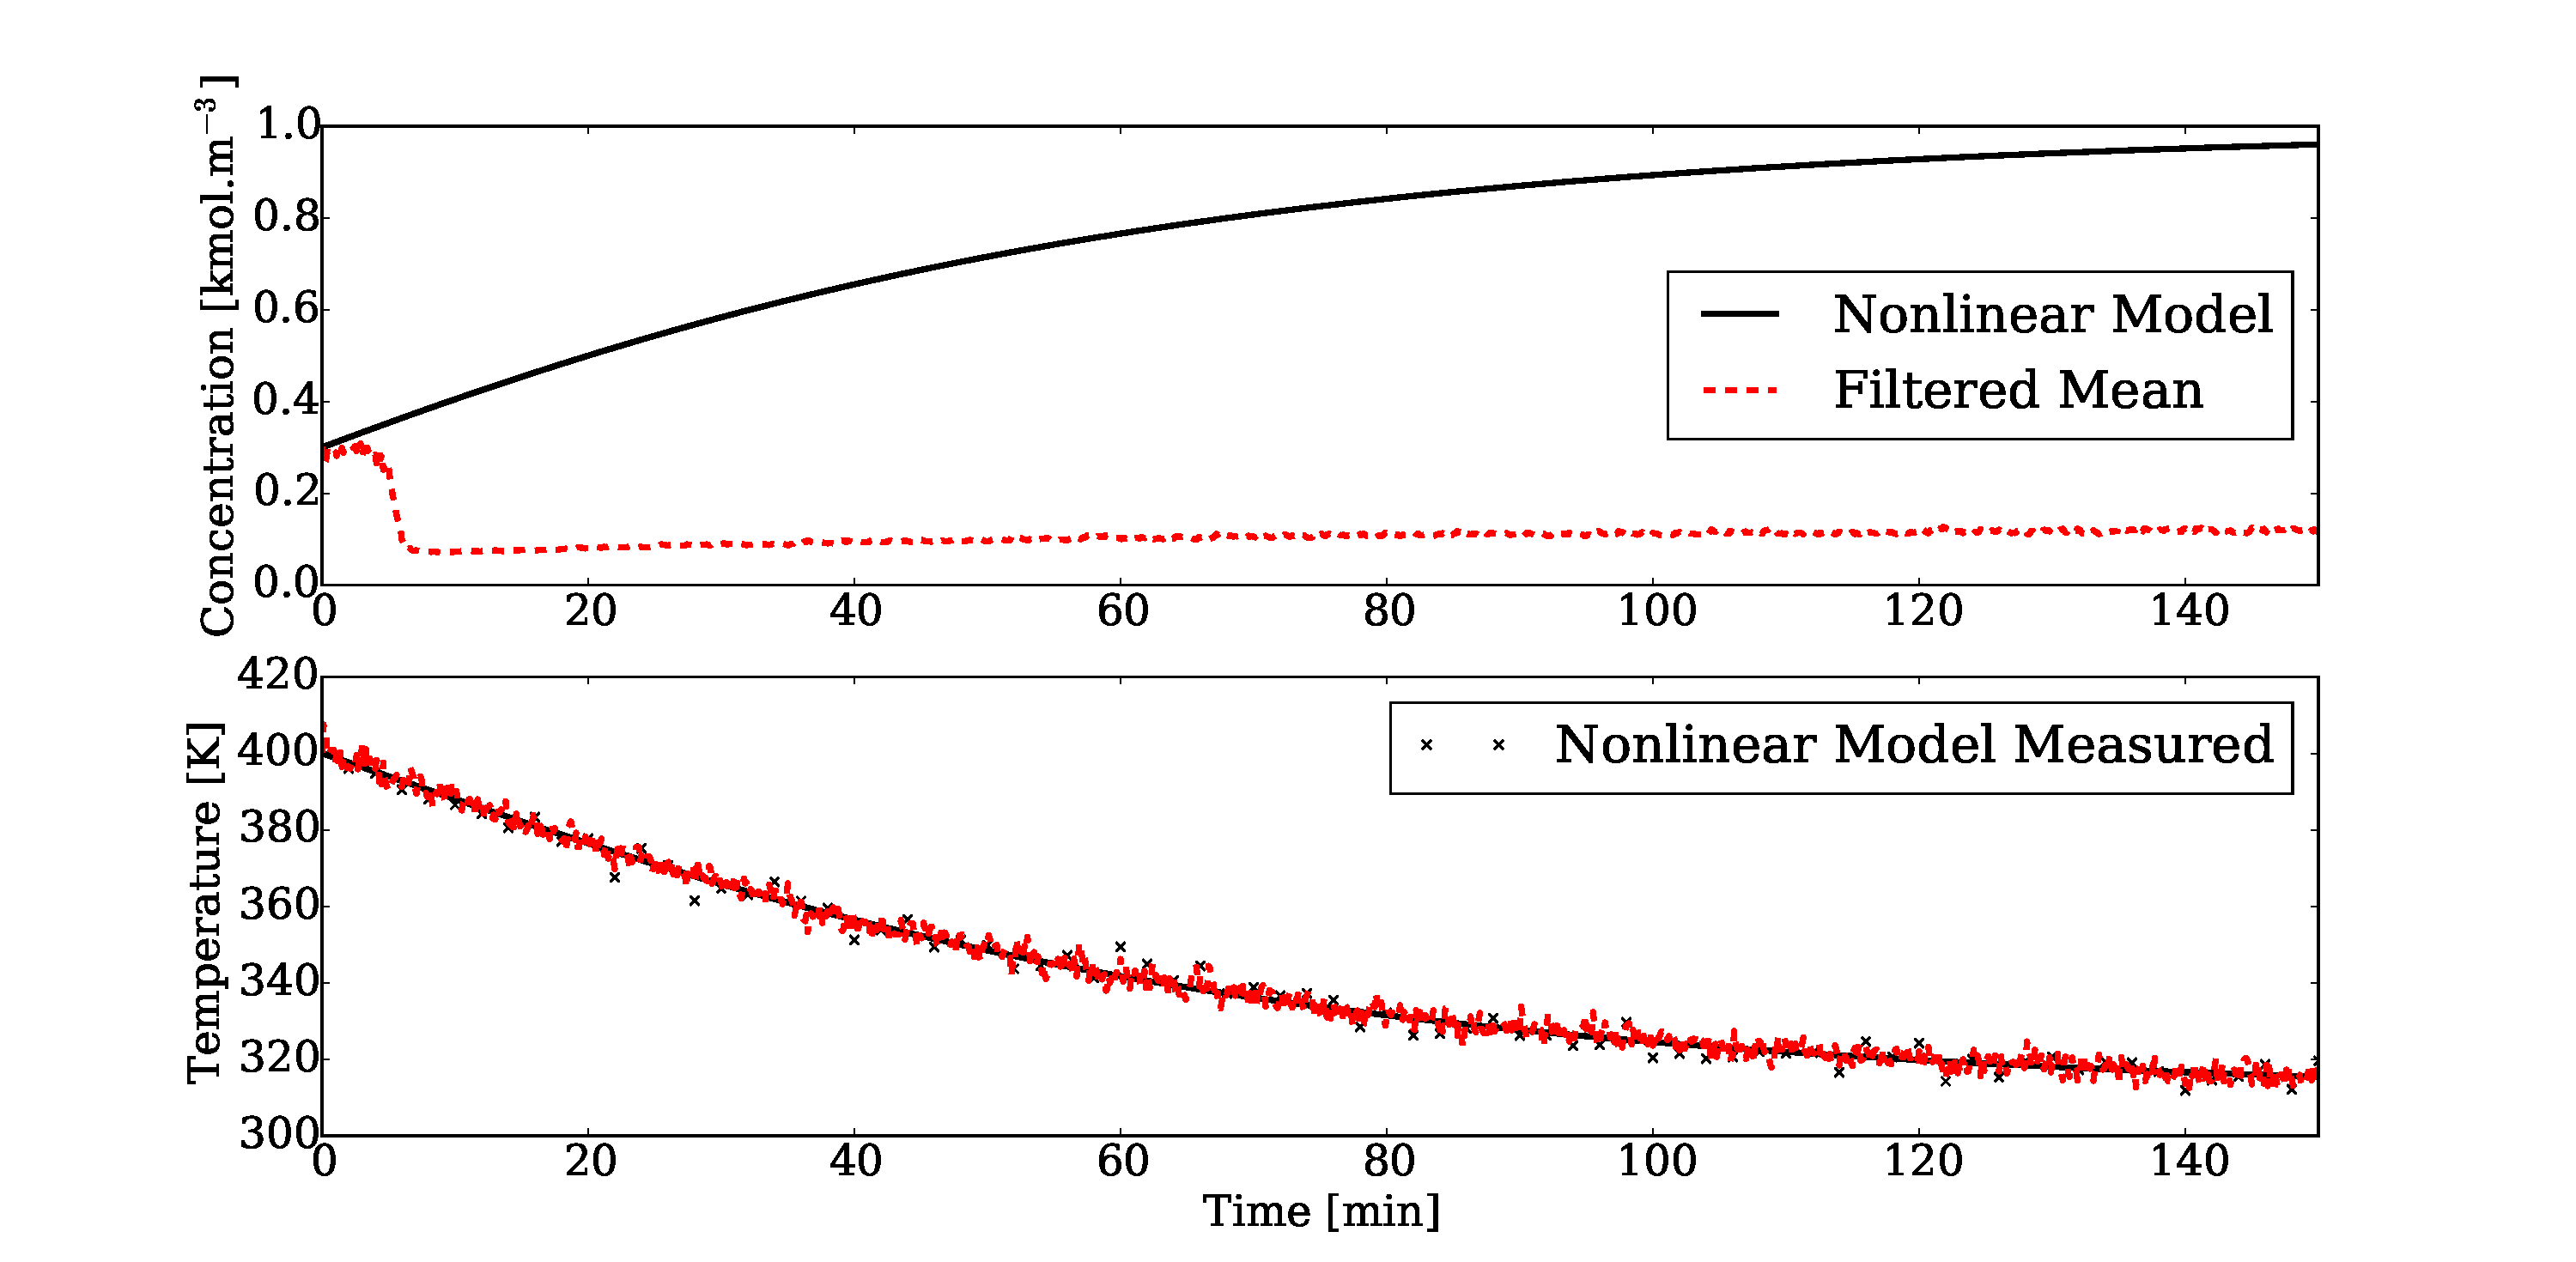
\includegraphics[scale=0.3]{skf_s3_t_w.pdf}
\caption{Time series evolution of the states with initial condition $(0.3, 400)$.}
\label{fig_3mod_t_w}
\end{figure}
Problems like this can be attenuated by using more particles or more linear models (or both). By trial and error we found that 7 linear models and 500 particles describes the system well while only measuring one state.

We now use 7 linear models to perform inference using the same initial conditions as Figure \ref{fig_3mod_t_w} to illustrate how increasing the number of linear models is beneficial to filtering accuracy. Figure \ref{fig_7mod_ss_m1} indicates that the lower temperature switches (models 1,3,6,7) should be most prominent during the run.  
\begin{figure}[H] 
\centering
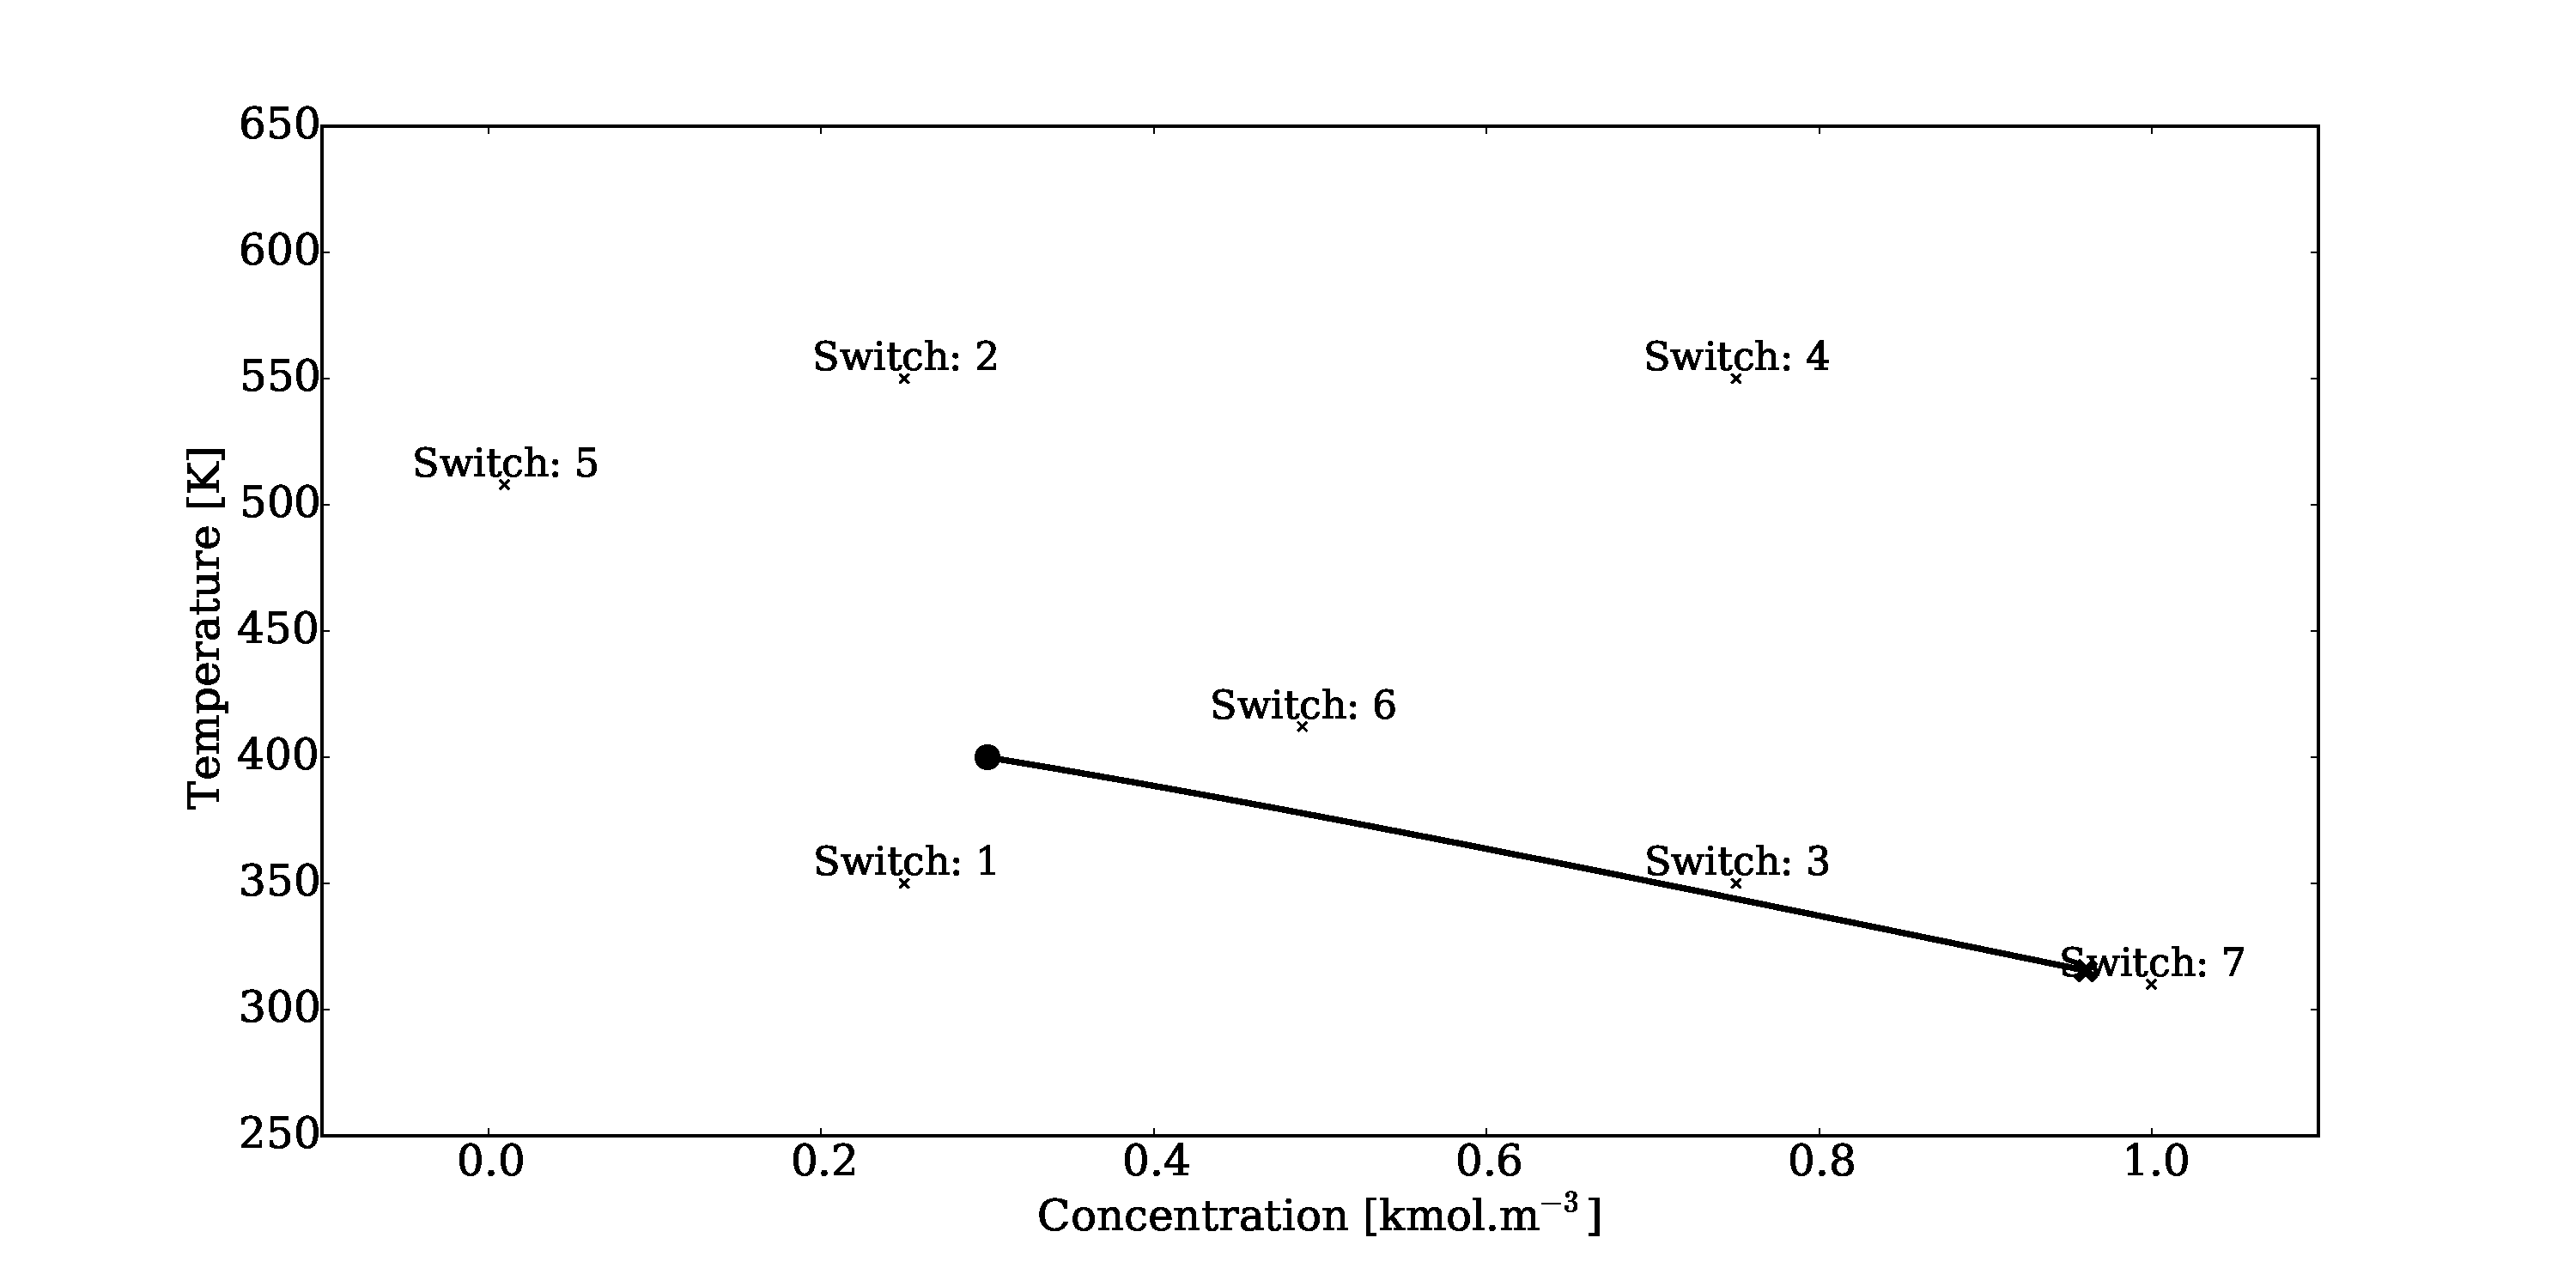
\includegraphics[scale=0.3]{skf_s7_s_m1.pdf}
\caption{State space evolution and linearisation points of the seven linear models used. The system starts at the black circle and ends at the black cross.}
\label{fig_7mod_ss_m1}
\end{figure}
In Figure \ref{fig_7mod_w_m1} we see that models 1,3,6 and 7 are indeed the most prominent models. This is reassuring because it indicates the filter correctly ``pick" the models which should best describe the system at each time step. 
\begin{figure}[H] 
\centering
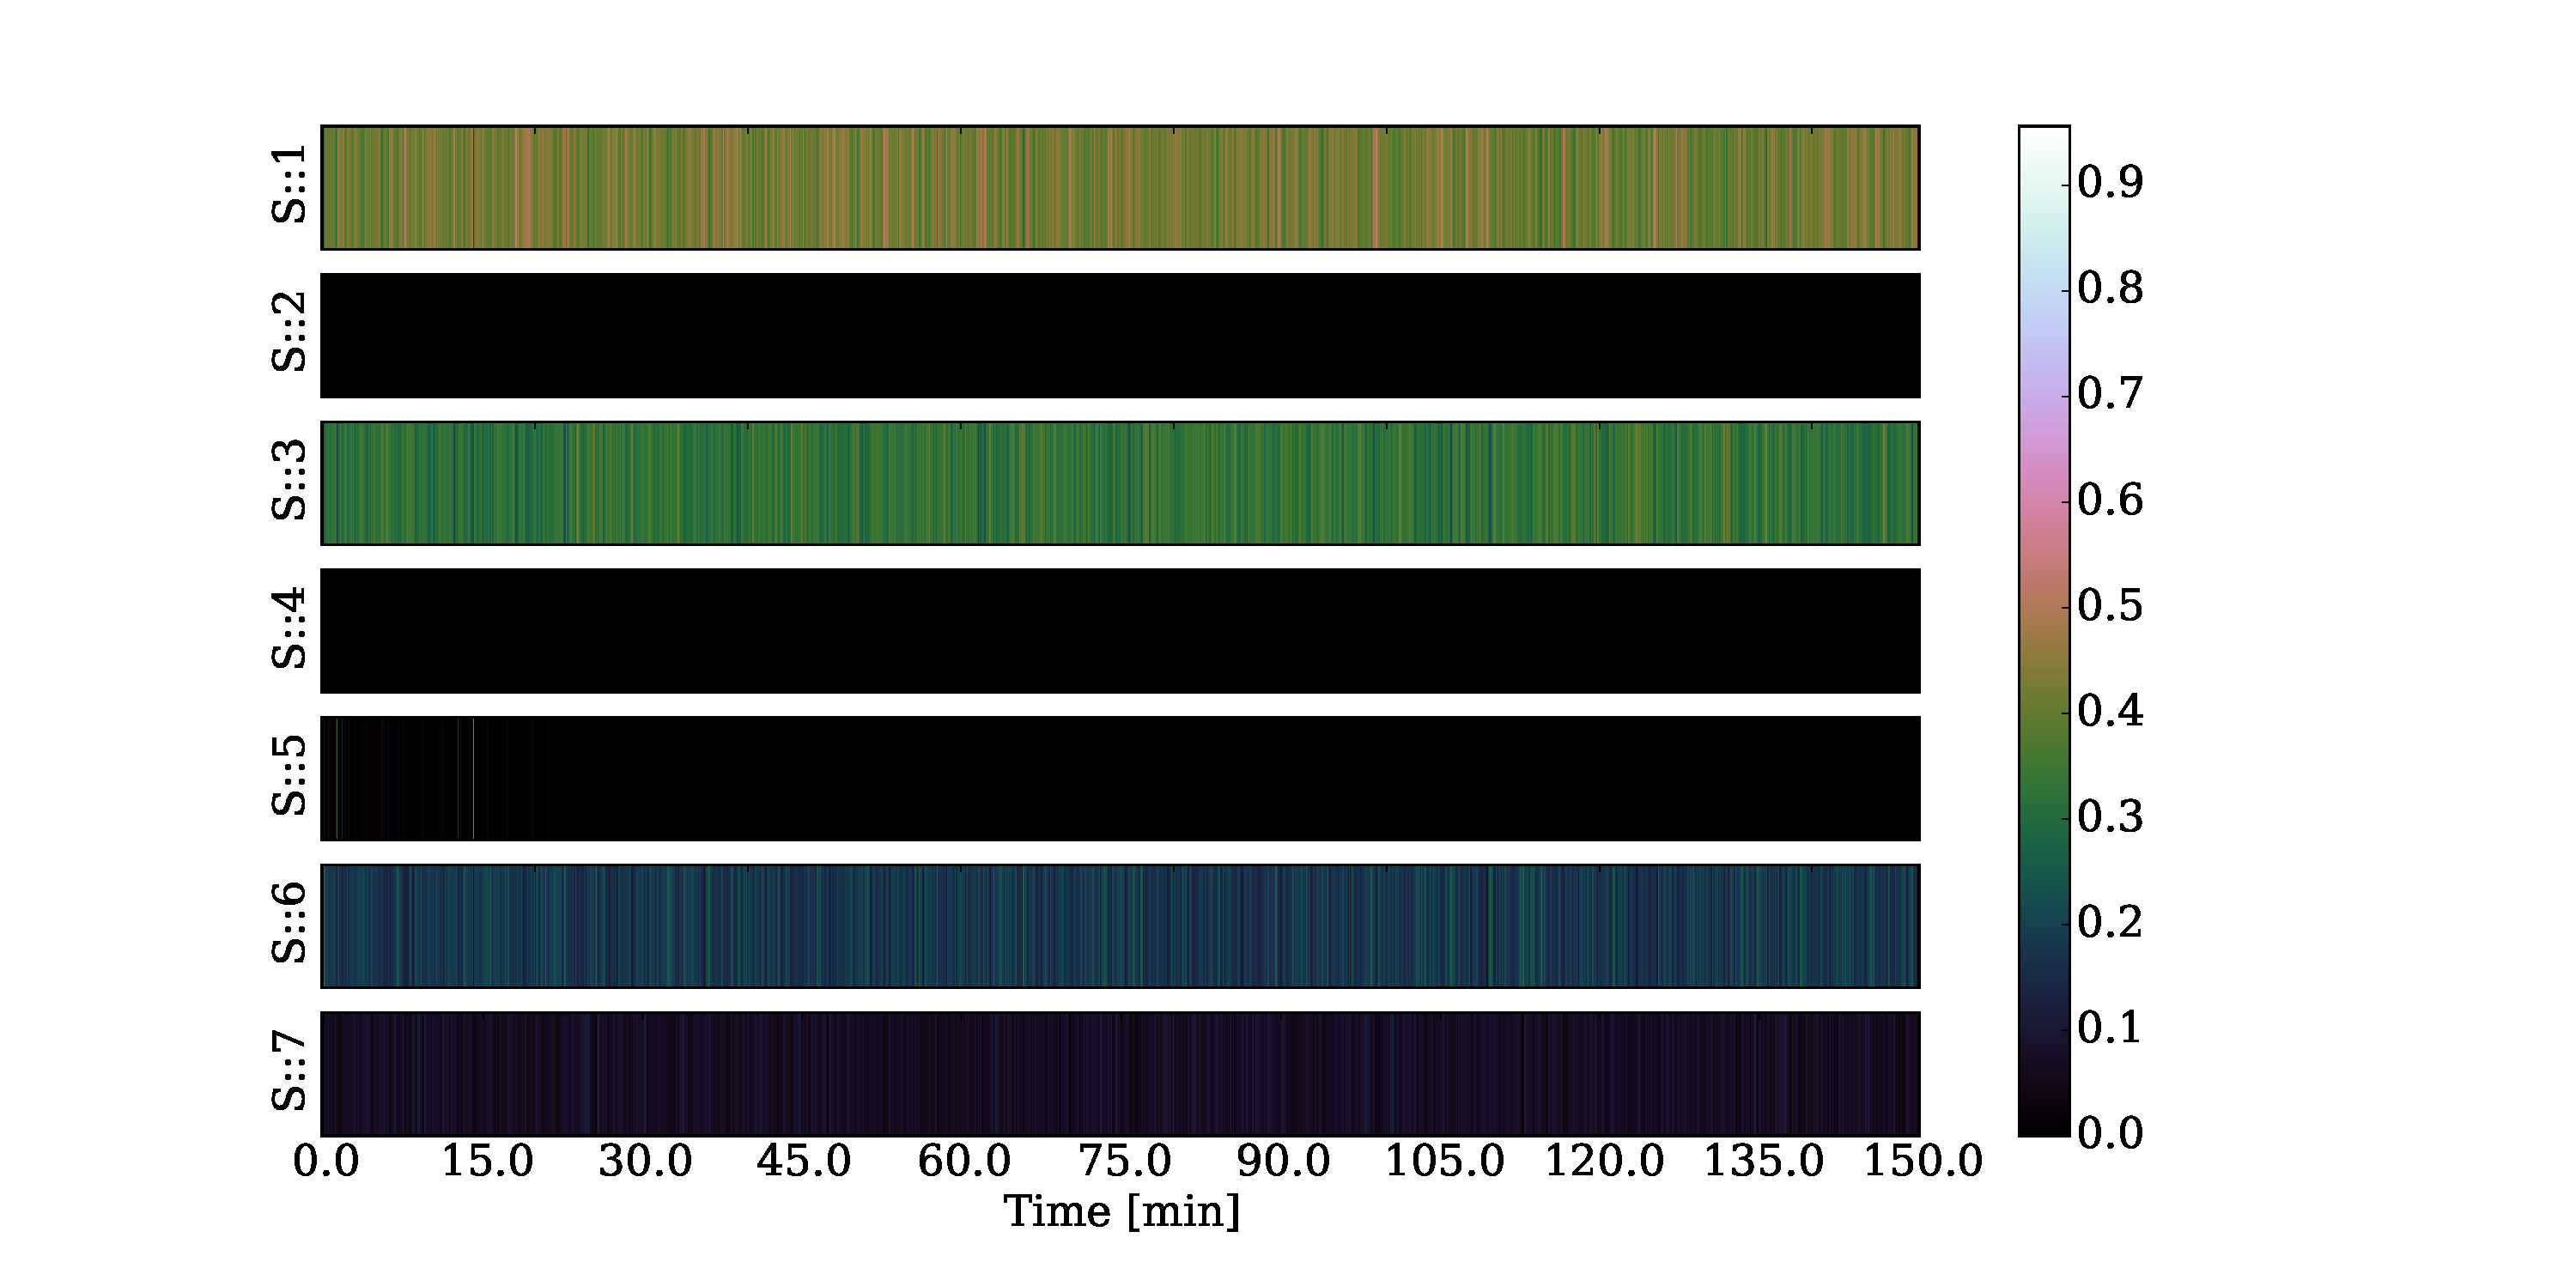
\includegraphics[scale=0.3]{skf_s7_w_m1.pdf}
\caption{Weight of each switching index as time progresses.}
\label{fig_7mod_w_m1}
\end{figure}
In Figure \ref{fig_7mod_t_m1} we see the filtered states as a function of time. We note that the temperature is accurately tracked but that there is almost a 20\% error in the concentration estimate. This is due to our single state measurement. Models 1 and 3 both predict the temperature of the system well but only model 3 predicts the concentration well. Since we do not measure concentration the filter has no way of knowing this and therefore includes a significant contribution of model 1 into the posterior state estimate. This causes the error we see in Figure \ref{fig_7mod_t_m1}.  
\begin{figure}[H] 
\centering
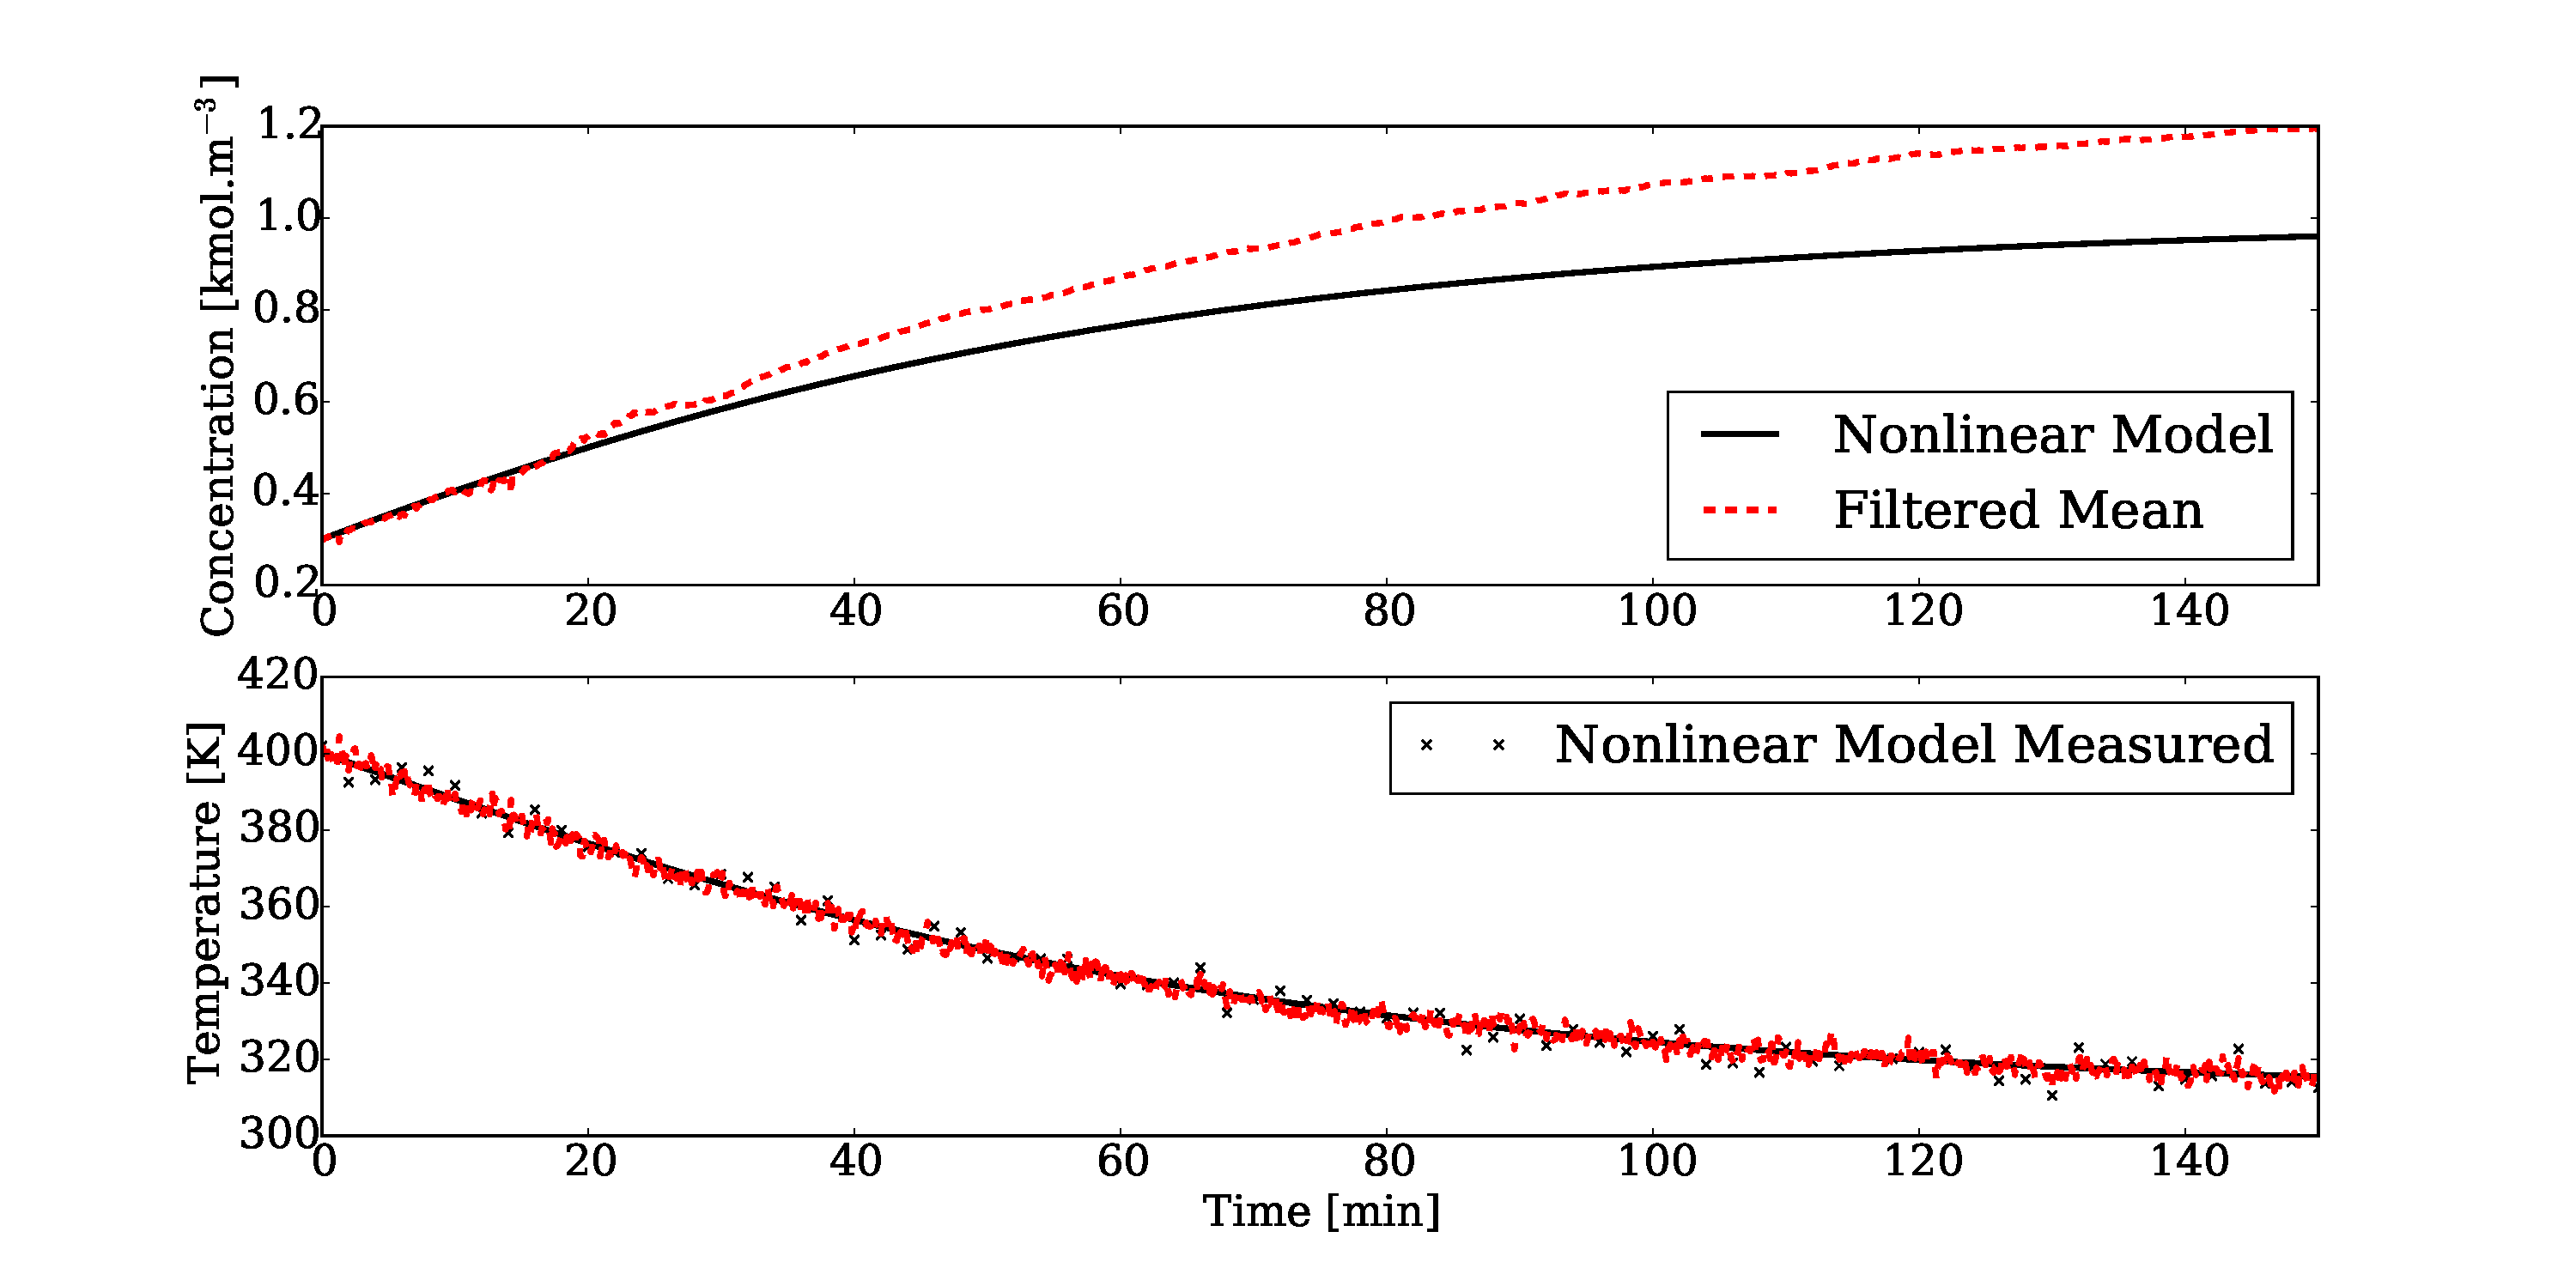
\includegraphics[scale=0.3]{skf_s7_t_m1.pdf}
\caption{Time series evolution of the states with initial condition $(0.3, 400)$.}
\label{fig_7mod_t_m1}
\end{figure}
The only way to eliminate the type  of error we see in Figure \ref{fig_7mod_t_m1} is to measure some facet of the concentration. In Figure \ref{fig_7mod_p_m1} we see the benefit of using the Switching Kalman Filter even when only measuring one state. The standard Kalman Filter used here was linearised about the unsteady operating point (model 6).
\begin{figure}[H] 
\centering
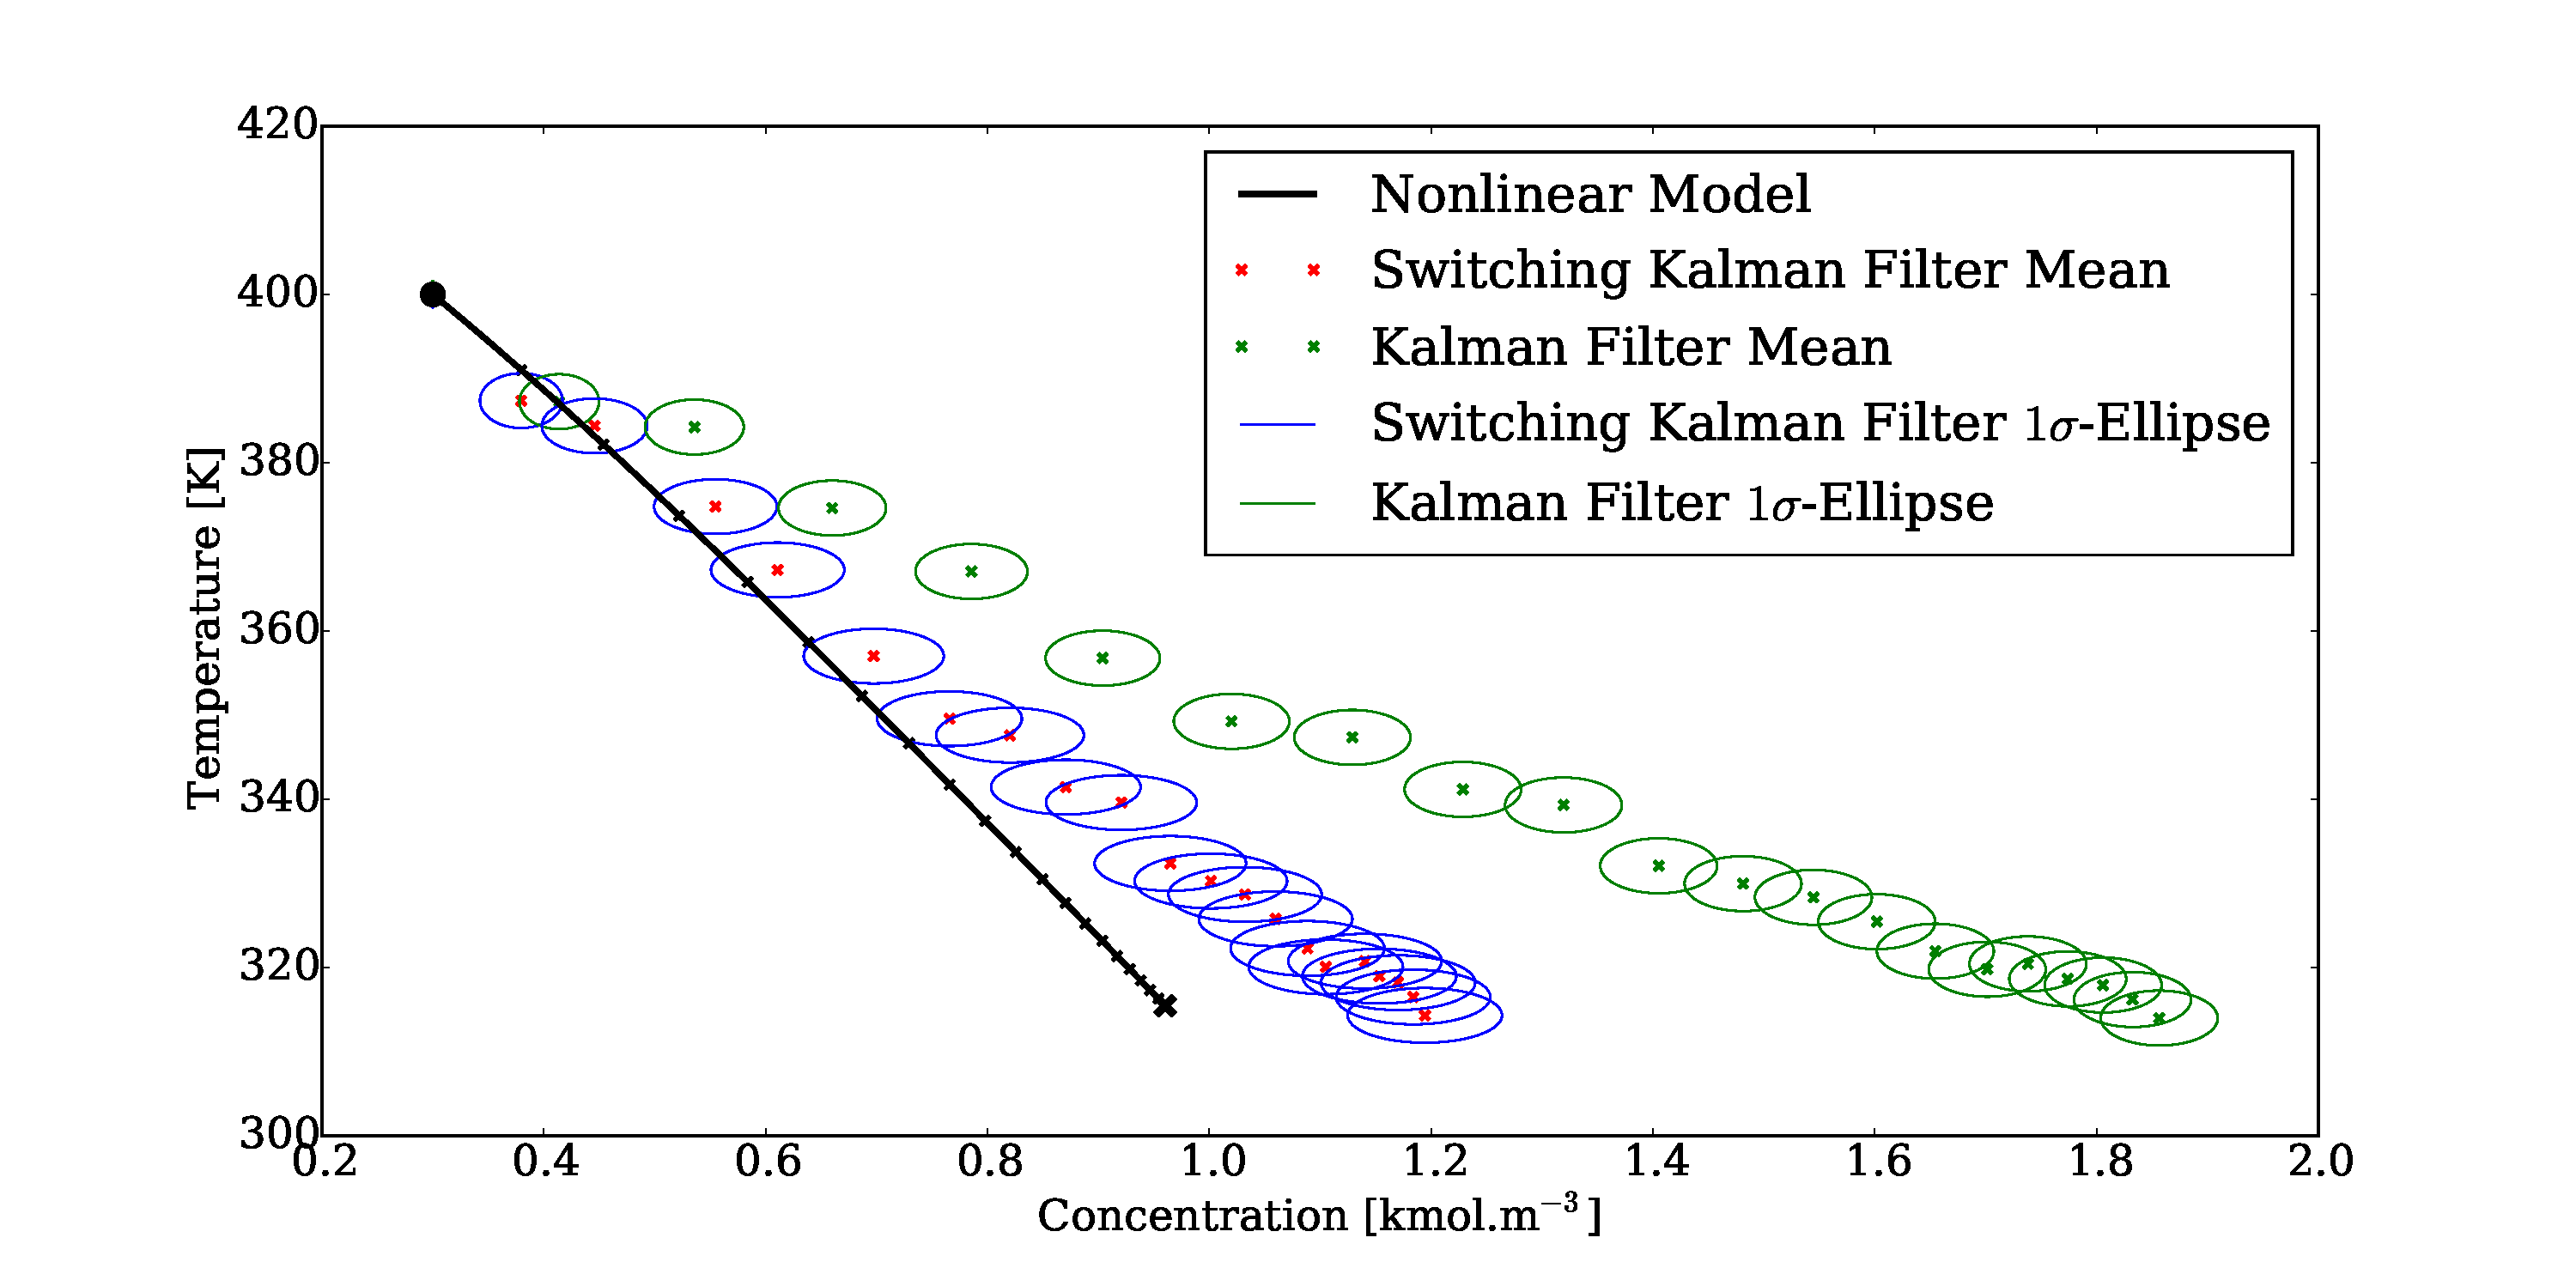
\includegraphics[scale=0.3]{skf_s7_p_m1.pdf}
\caption{State space evolution of the Switching Kalman Filter and the standard Kalman filter which only uses one linear model.}
\label{fig_7mod_p_m1}
\end{figure}
As discussed before, the standard Kalman Filter poorly estimates the unmeasured state because the linear model is uses is not accurate throughout the state space. However, the Switching Kalman Filter can switch models so that poor models do not form part of its state estimate. Thus it is better able to track the unmeasured state estimate.  

As mentioned in the preceding discussion, measuring only one state can cause inaccurate state estimates. It is always better (perhaps not in an economic sense) to measure as much as possible for the purposes of inference. In Figures \ref{fig_7mod_ss_m2} to \ref{fig_7mod_p_m2} we incorporate a concentration measurement to improve inference. 

In Figure \ref{fig_7mod_ss_m2} we see the trajectory of the state evolution in state space. From this we expect models 1,3,6 and 7 to be active. 
\begin{figure}[H] 
\centering
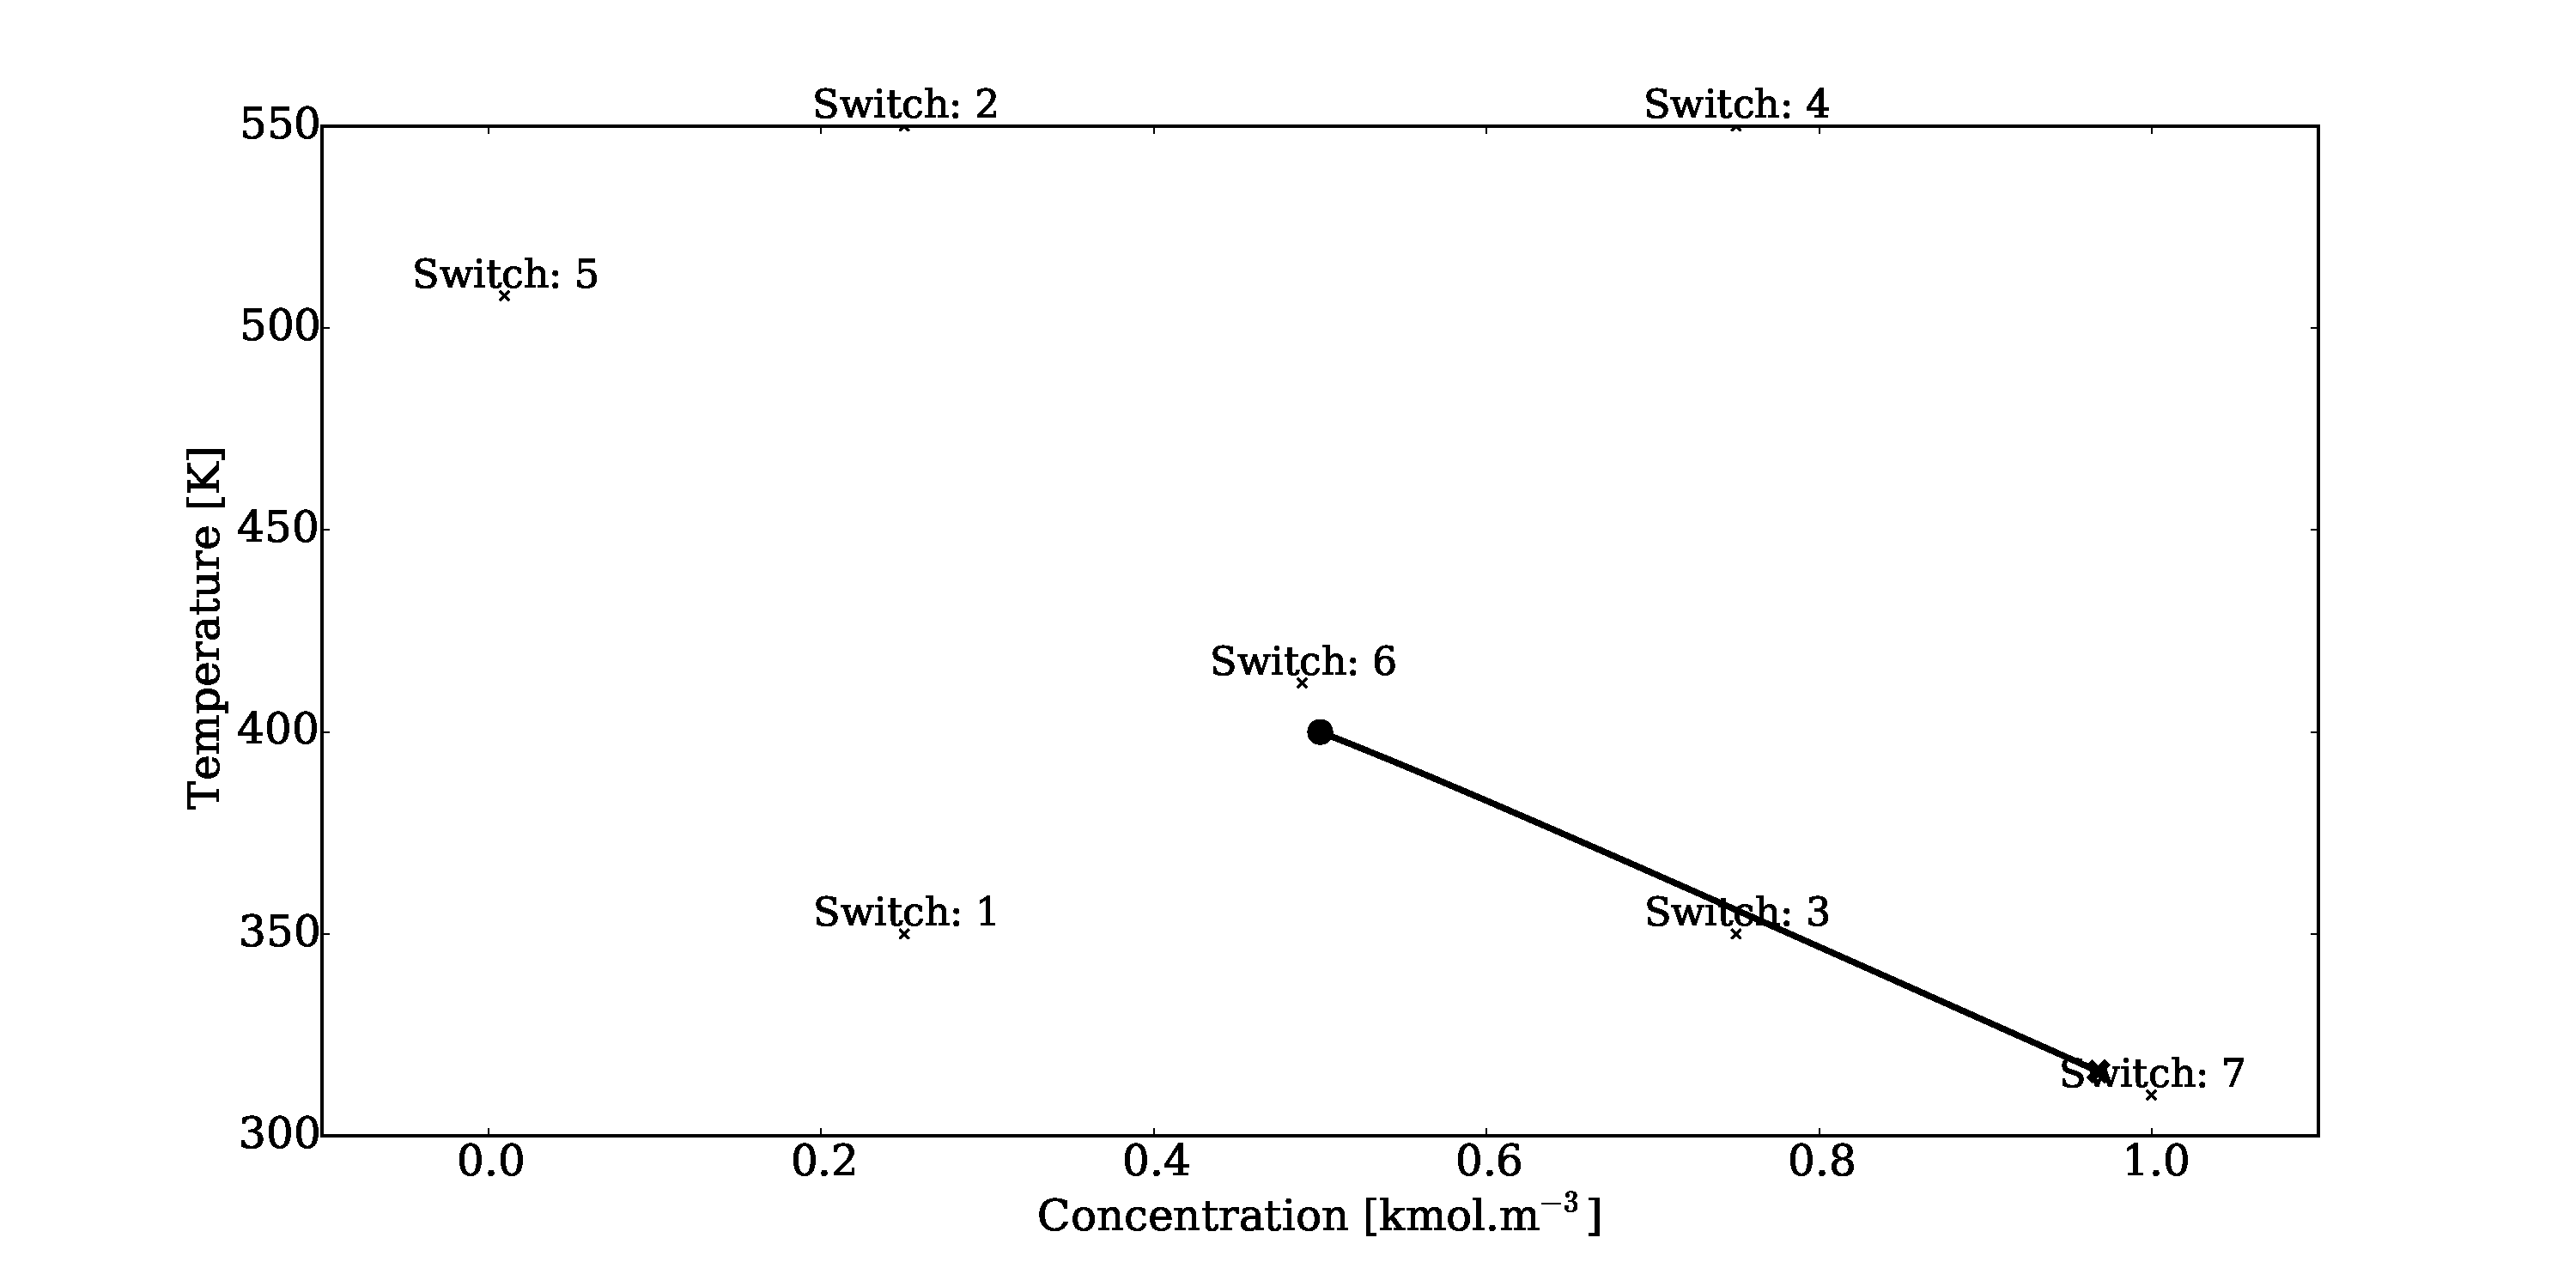
\includegraphics[scale=0.3]{skf_s7_s_m2.pdf}
\caption{State space evolution and linearisation points of the three linear models used. The system starts at the black circle and ends at the black cross.}
\label{fig_7mod_ss_m2}
\end{figure}
In Figure \ref{fig_7mod_w_m2} we see that indeed models 1,3,6 and 7 are active. This indicates that the filter is likely to track the states well because the more accurate models are used for inference.
\begin{figure}[H] 
\centering
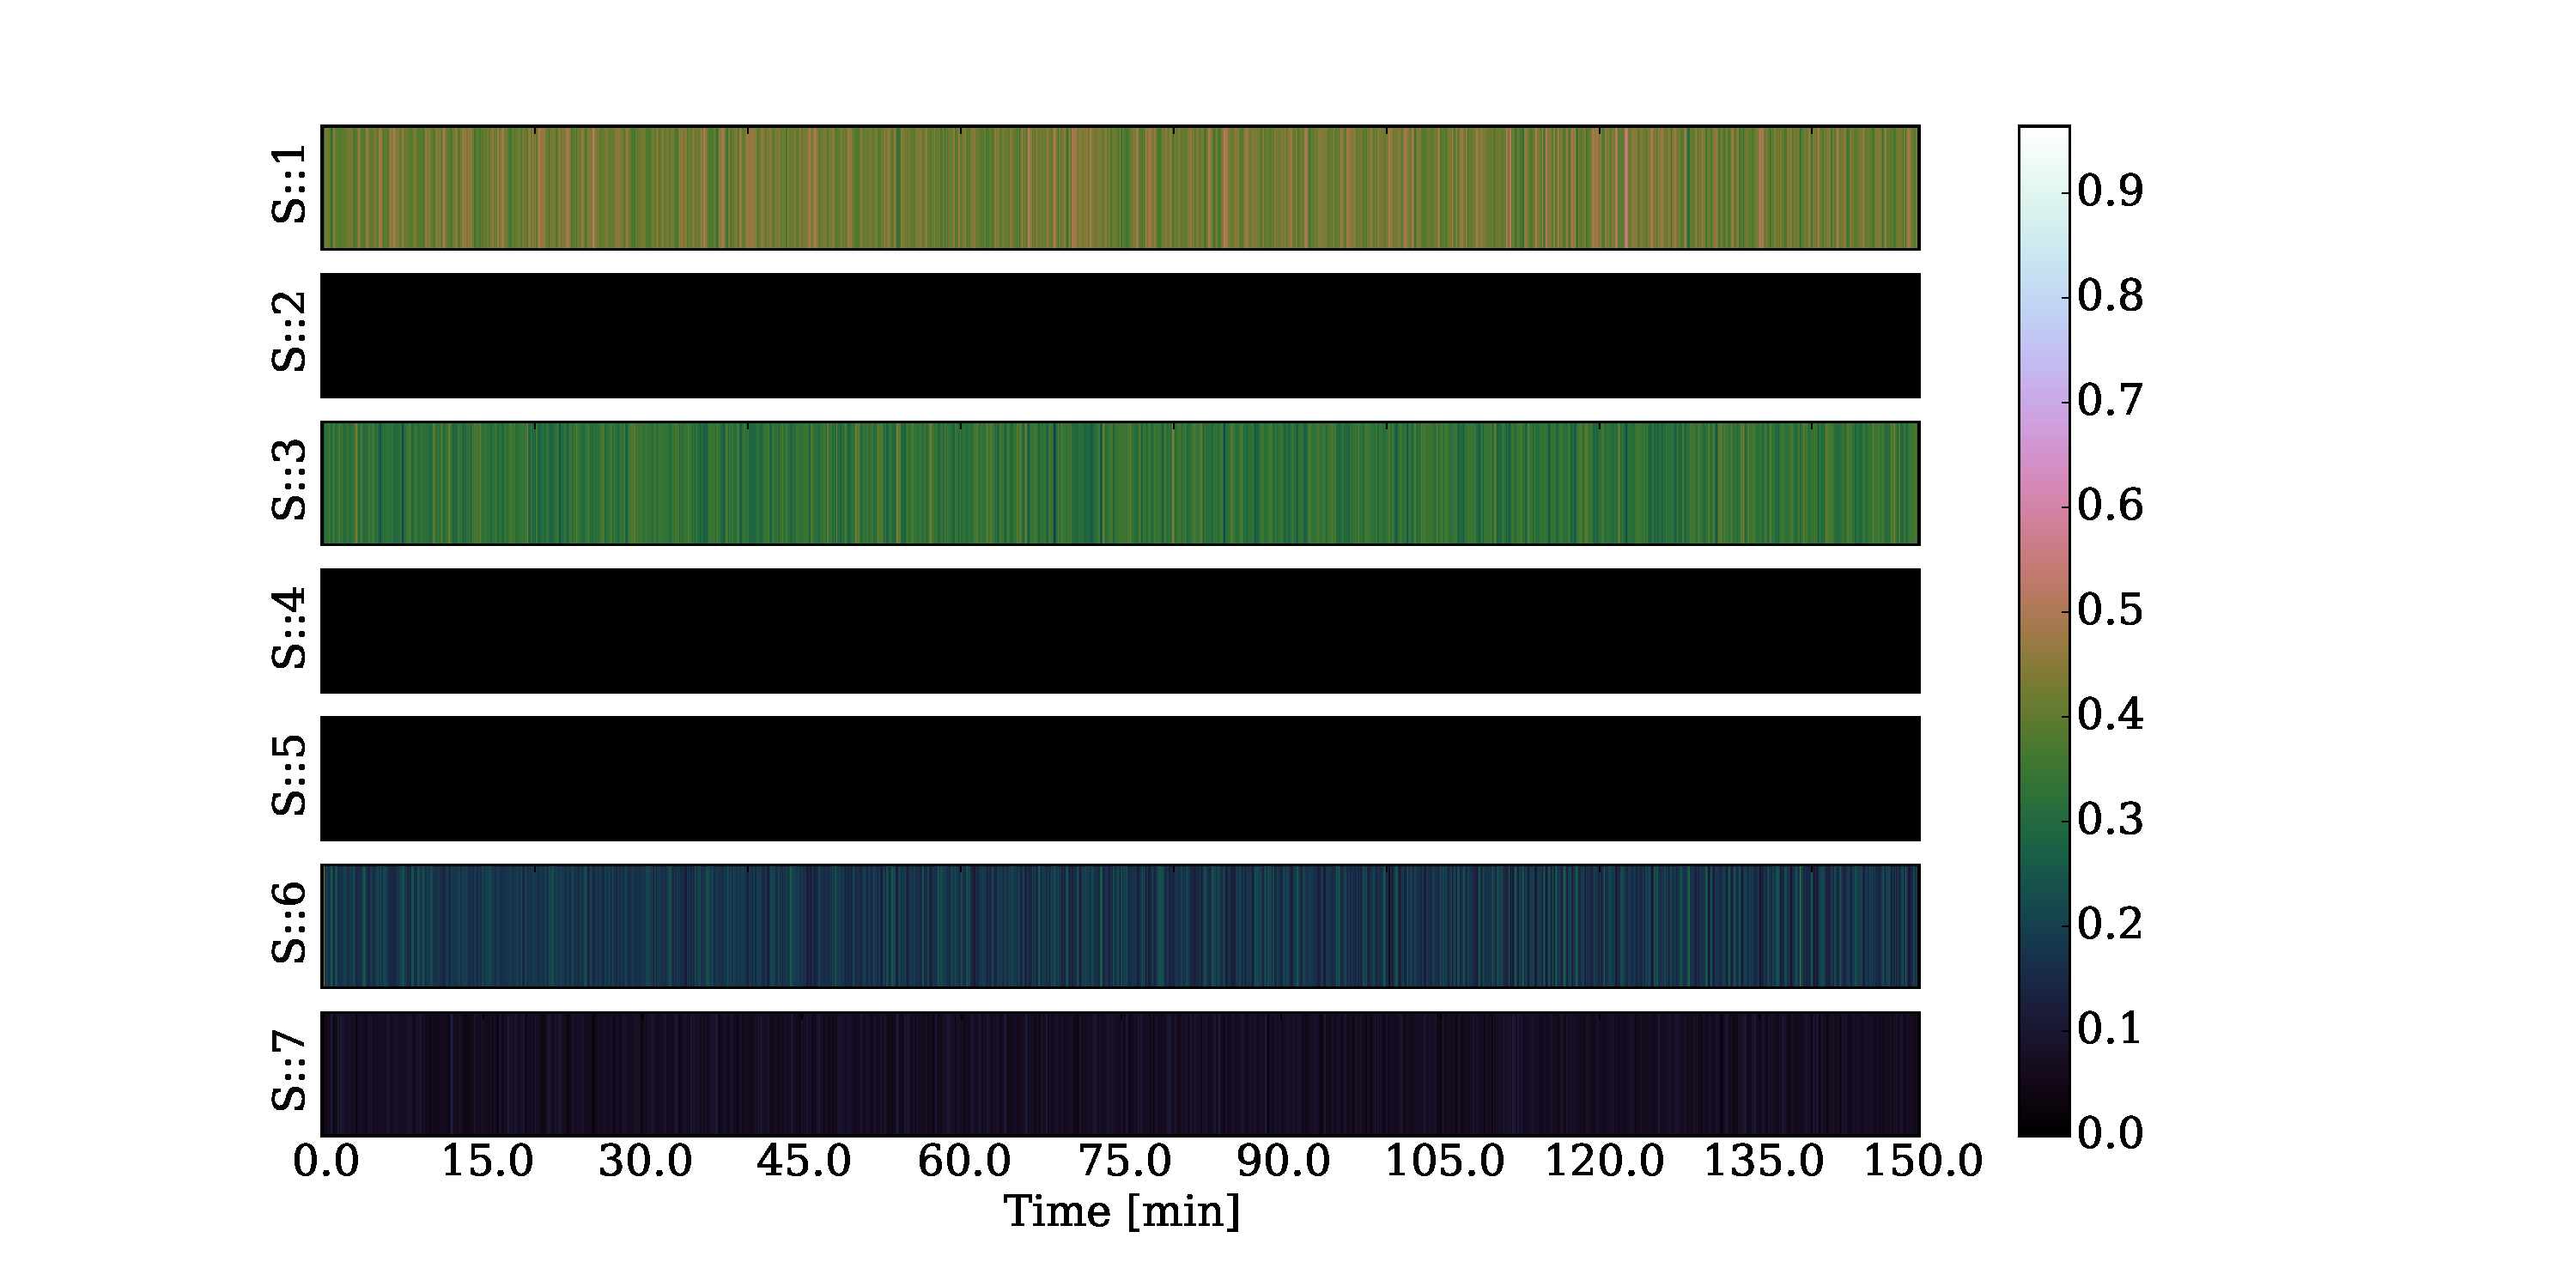
\includegraphics[scale=0.3]{skf_s7_w_m2.pdf}
\caption{Weight of each switching index as time progresses.}
\label{fig_7mod_w_m2}
\end{figure}
In Figure \ref{fig_7mod_t_m2} we see that indeed the filter accurately tracks both concentration and temperature. At this stage it becomes important to question if the Switching Kalman Filter increased the accuracy of the state estimate. After all, the standard Kalman Filter also accurately tracked both states given both measurements and was computationally much less intensive than the Switching Kalman Filter. 
\begin{figure}[H] 
\centering
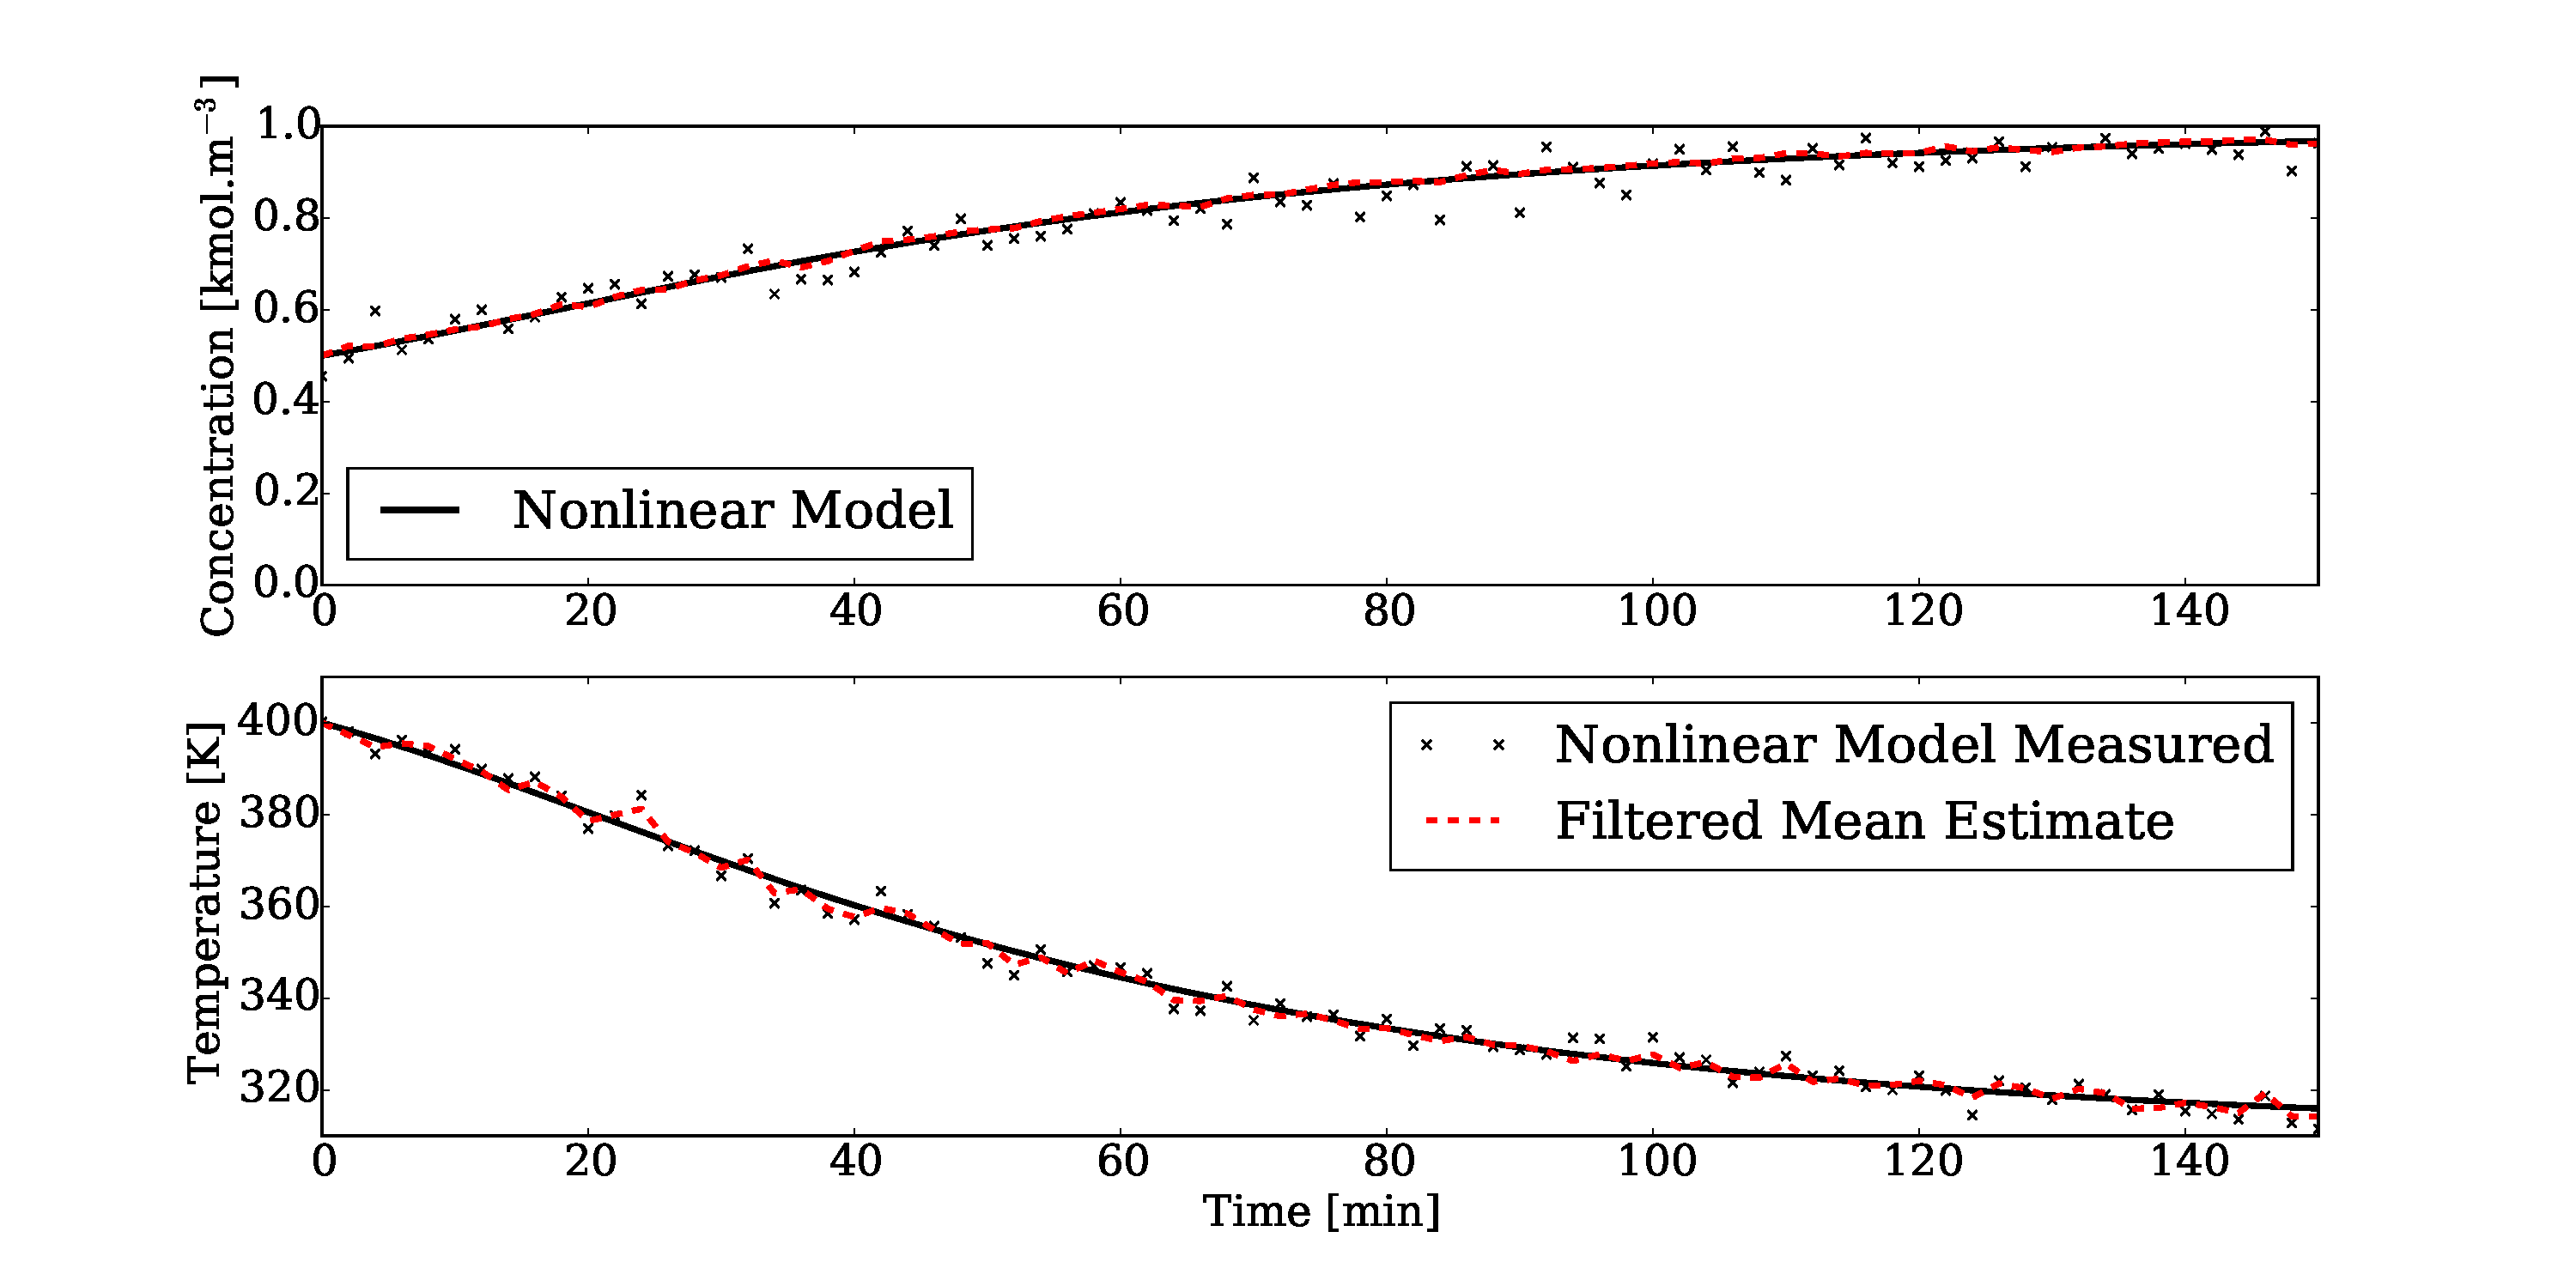
\includegraphics[scale=0.3]{skf_s7_t_m2.pdf}
\caption{Time series evolution of the states with initial condition $(0.5, 400)$.}
\label{fig_7mod_t_m2}
\end{figure}
In Figure \ref{fig_7mod_p_m2} we compare the Switching Kalman Filter to the standard Kalman Filter which uses only model 6.
\begin{figure}[H] 
\centering
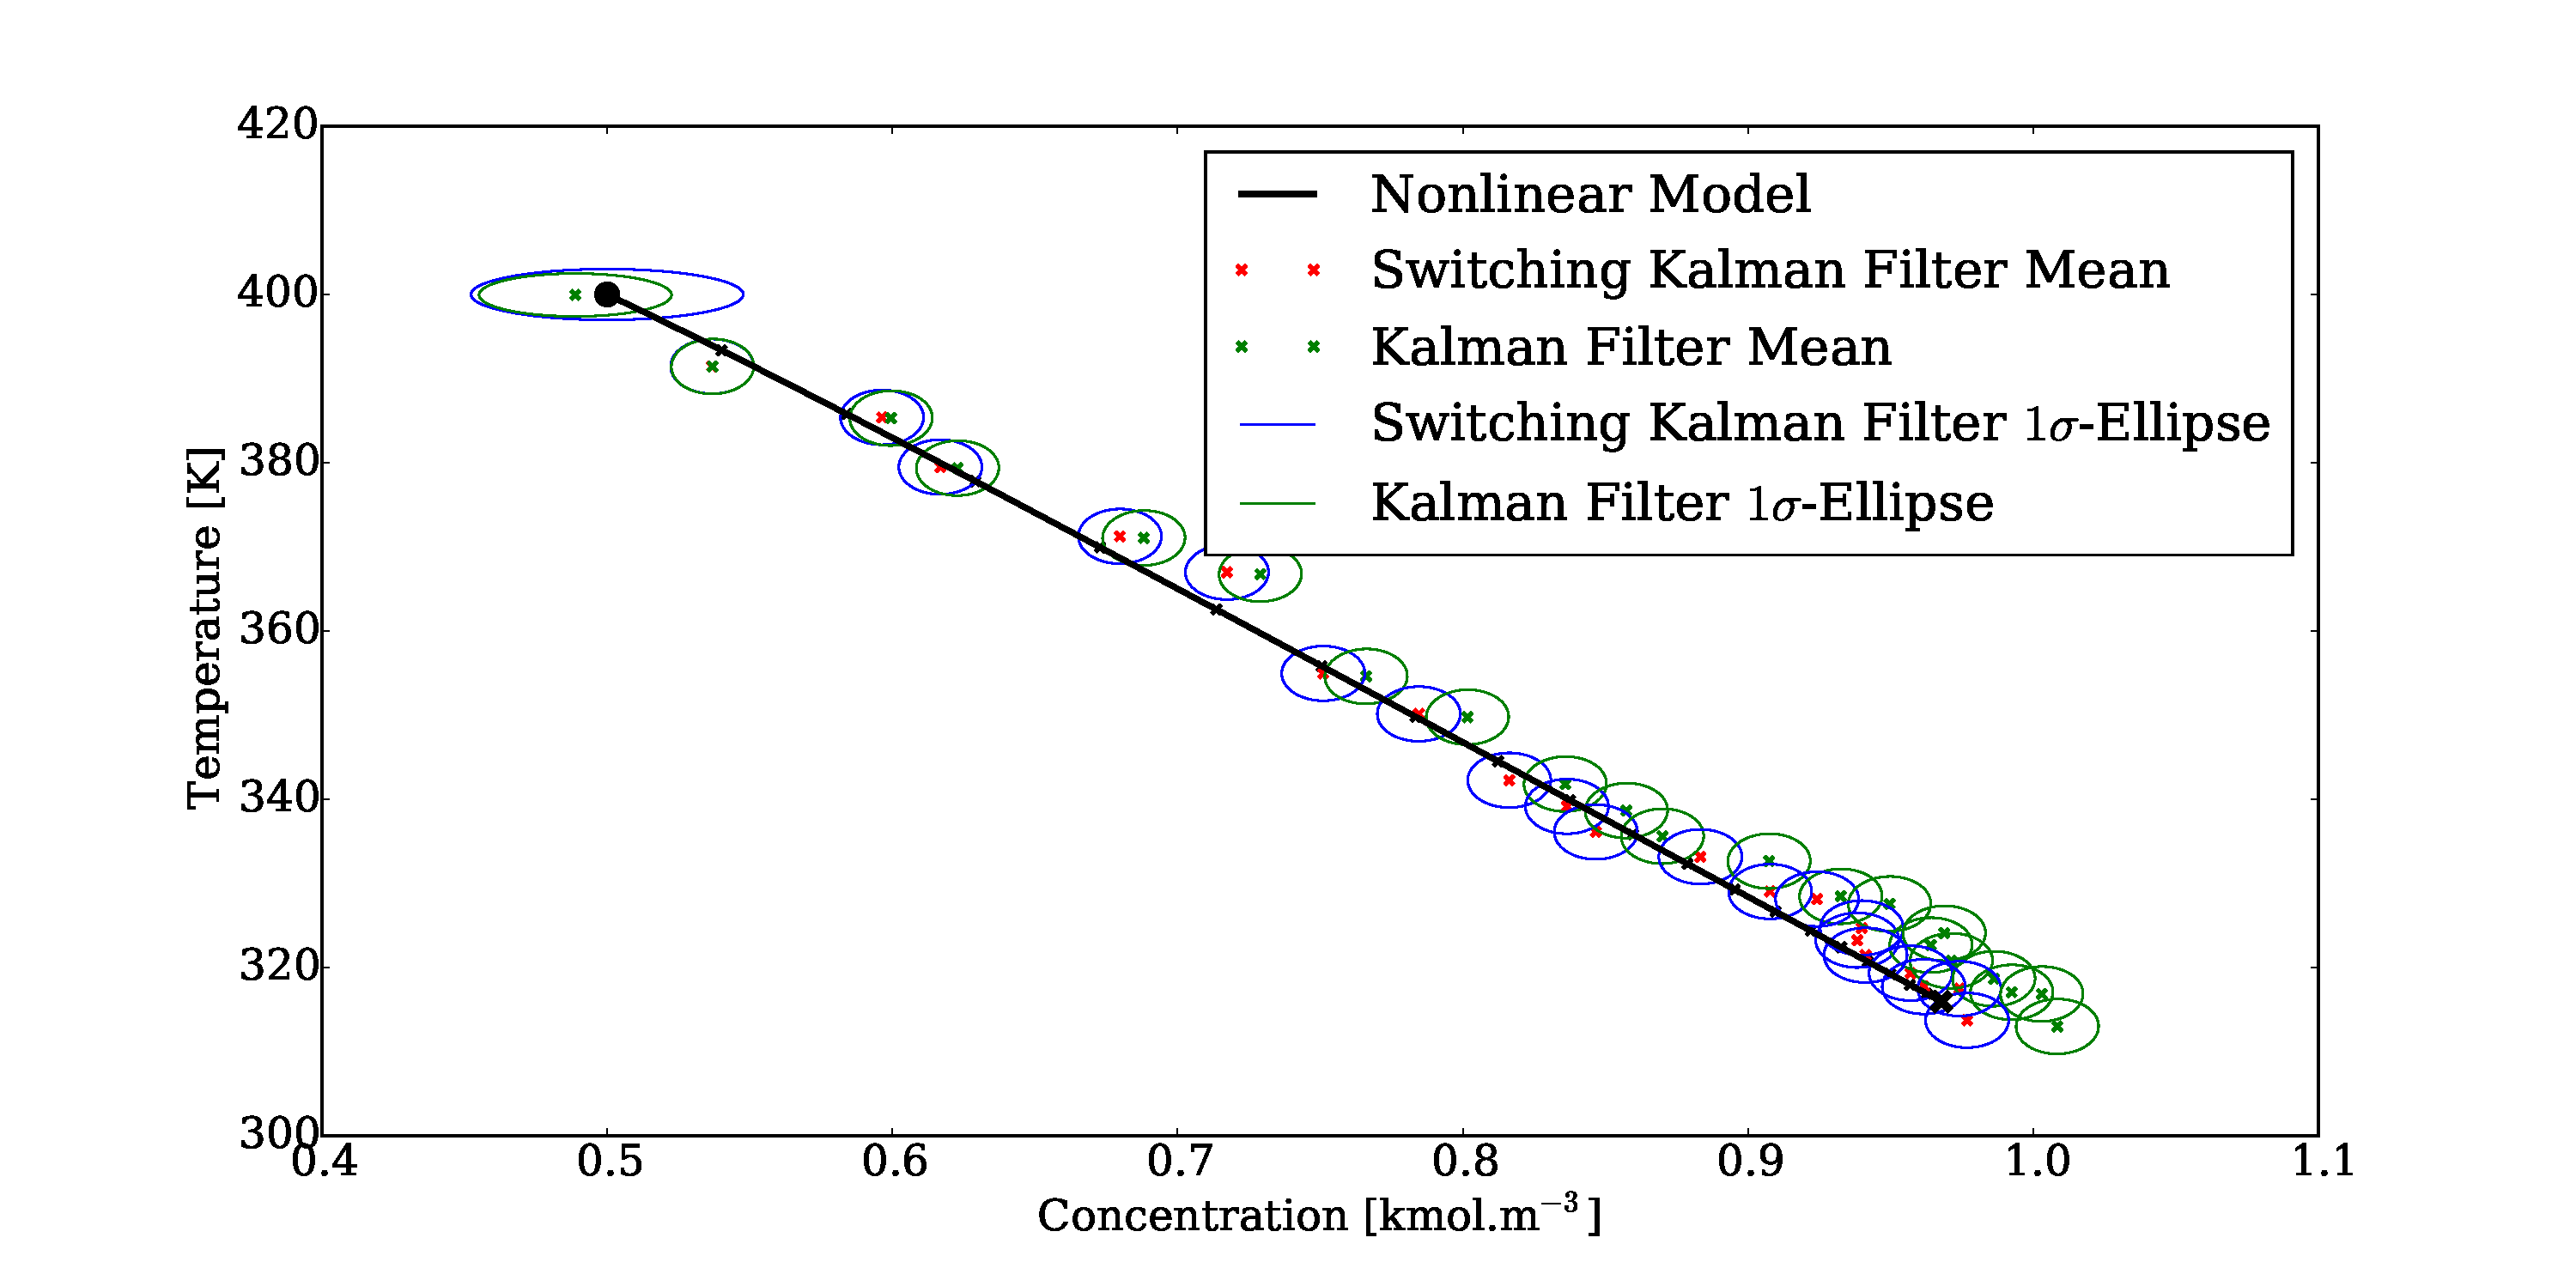
\includegraphics[scale=0.3]{skf_s7_p_m2.pdf}
\caption{State space evolution of the Switching Kalman Filter and the standard Kalman filter which only uses one linear model.}
\label{fig_7mod_p_m2}
\end{figure}
Based on Figure \ref{fig_7mod_p_m2} we see that there is some benefit in using the Switching Kalman Filter. However, this is less pronounced than when only one state is measured (see Figure \ref{fig_7mod_p_m1}). The reason is: the standard Kalman Filter eventually only uses the measurements to infer the posterior state estimates because the model is bad. Thus the accuracy of the standard Kalman Filter will depend strongly the magnitude of the measurement noise. However, the Switching Kalman Filter can depend on the models to a much greater extent and we thus expect large measurement noise to not affect the quality of the state estimate as much. 

To illustrate this effect we increase the measurement noise significantly: $R=\begin{pmatrix}
0.1 & 0 \\ 0 & 100
\end{pmatrix}$. The results are shown in Figures  \ref{fig_7mod_t_m2_b} to \ref{fig_7mod_p_m2_b}. We see in Figure \ref{fig_7mod_t_m2_b} that the measurement noise is significantly worse but the filter still tracks the states reliably.
\begin{figure}[H] 
\centering
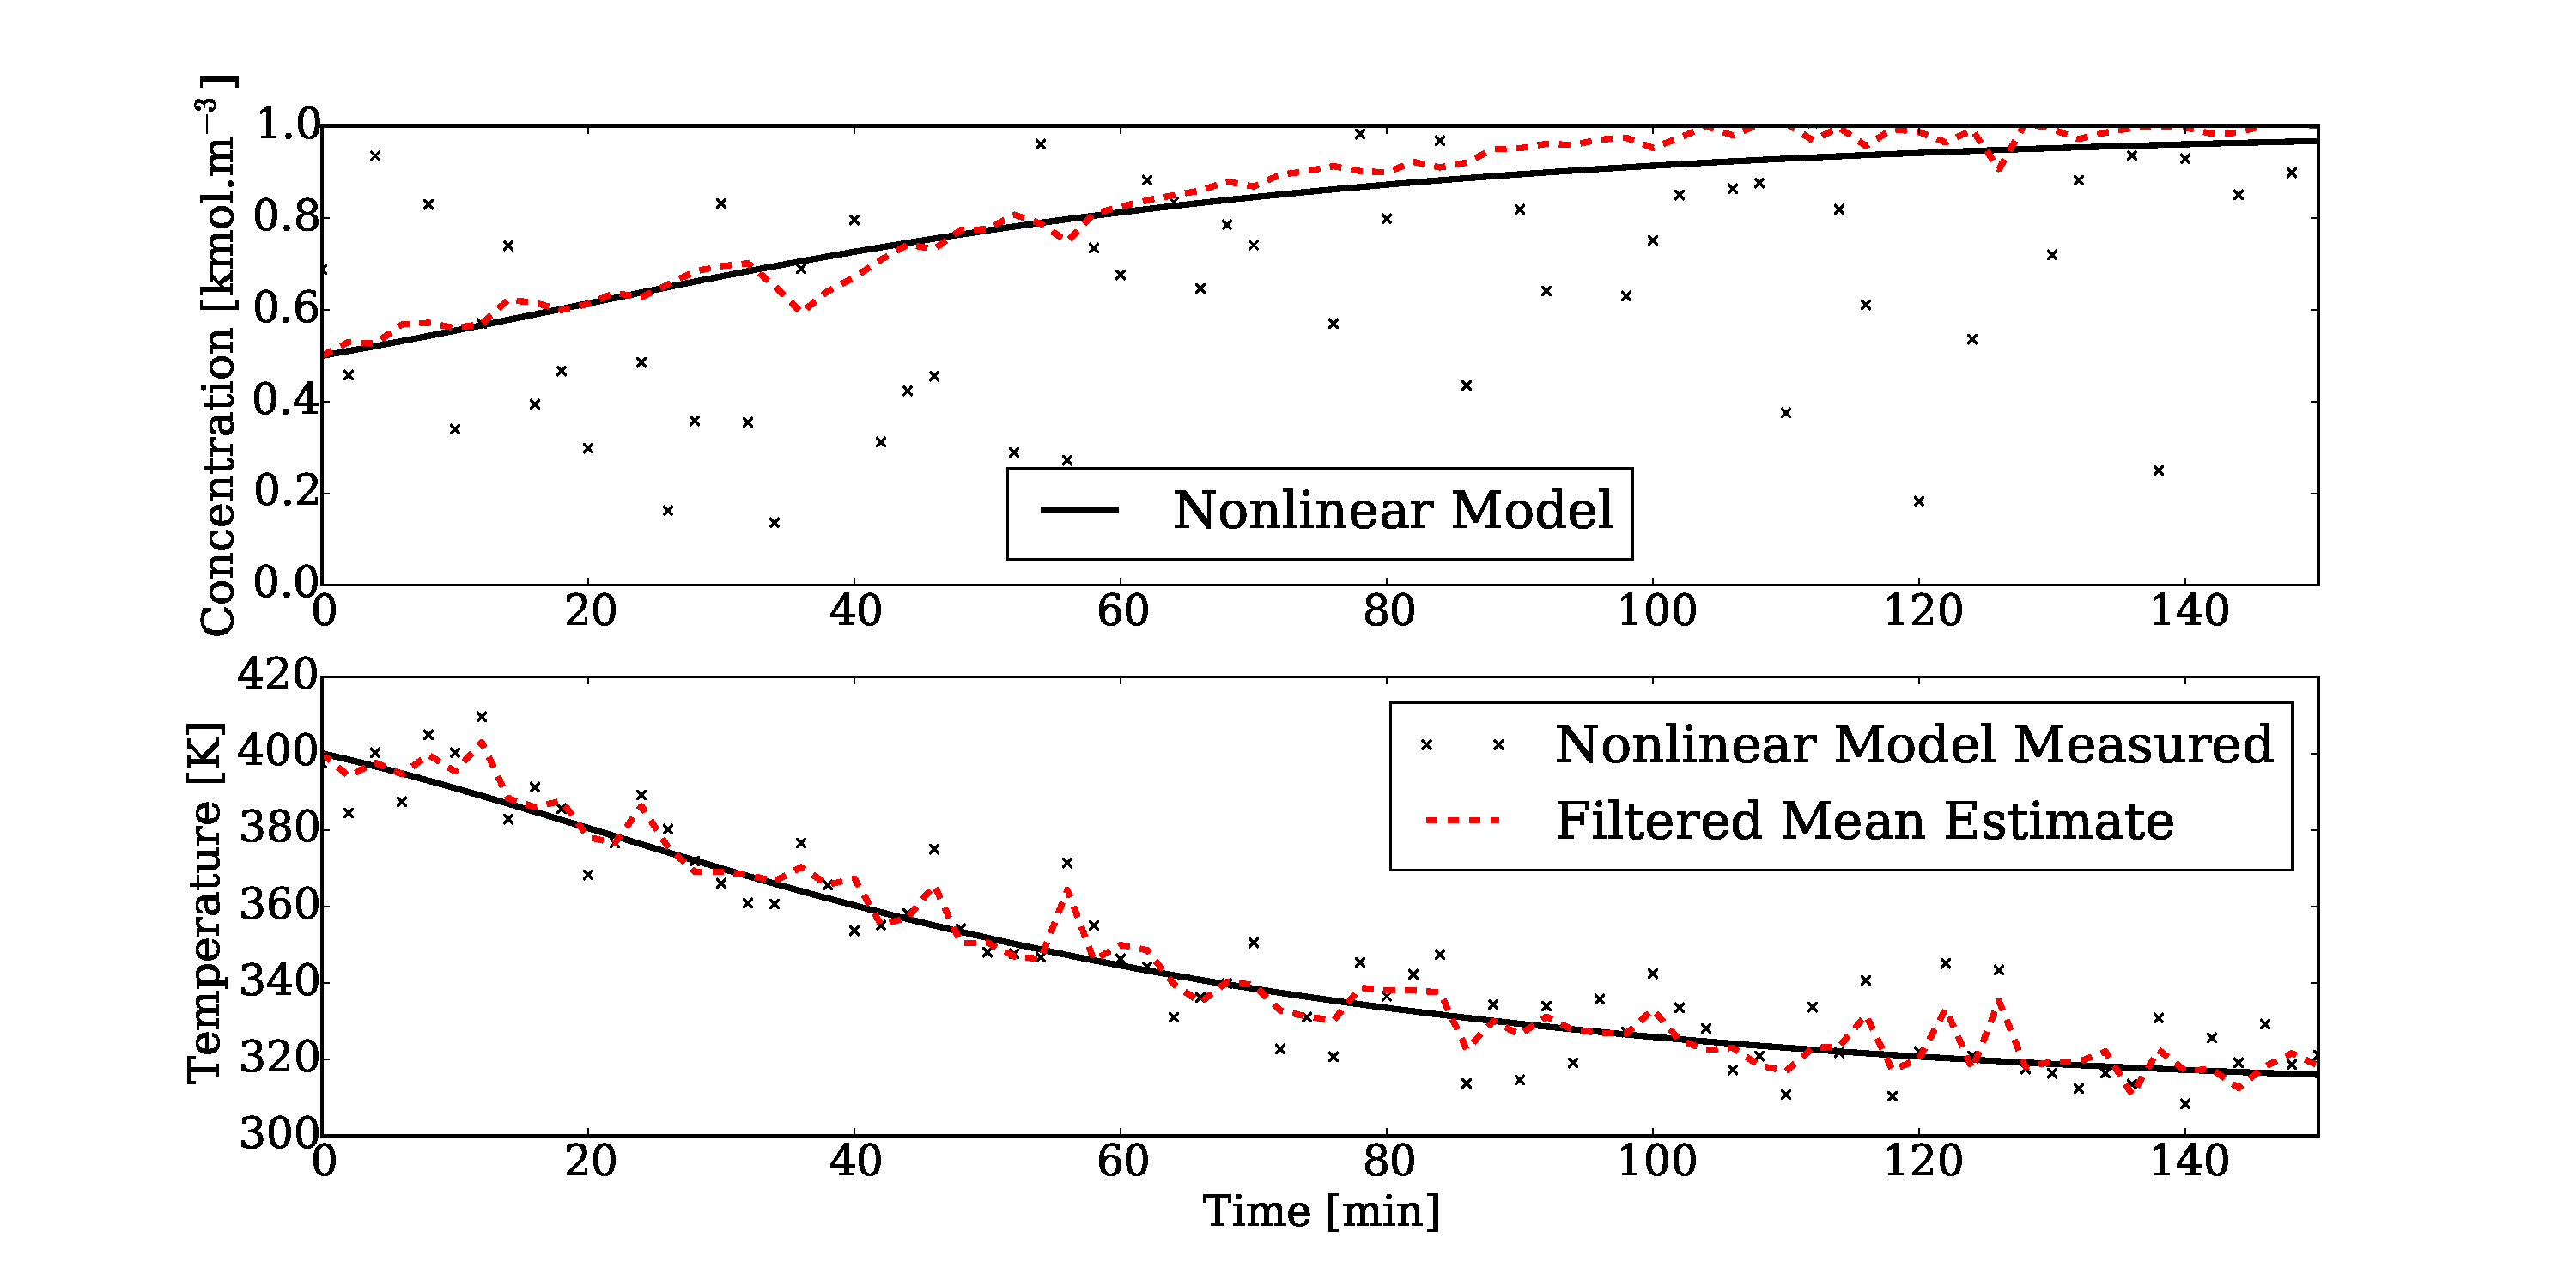
\includegraphics[scale=0.3]{skf_s7_t_m2_b.pdf}
\caption{Time series evolution of the states with initial condition $(0.5, 400)$ and using a much larger noise covariance.}
\label{fig_7mod_t_m2_b}
\end{figure}
However, in Figure \ref{fig_7mod_p_m2_b} we see that the standard Kalman Filter does not track the states well. Since the model is bad the standard Kalman Filter has to rely on measurements which are also bad, hence the poor performance. The Switching Kalman Filter does not have this problem and is significantly more reliable.
\begin{figure}[H] 
\centering
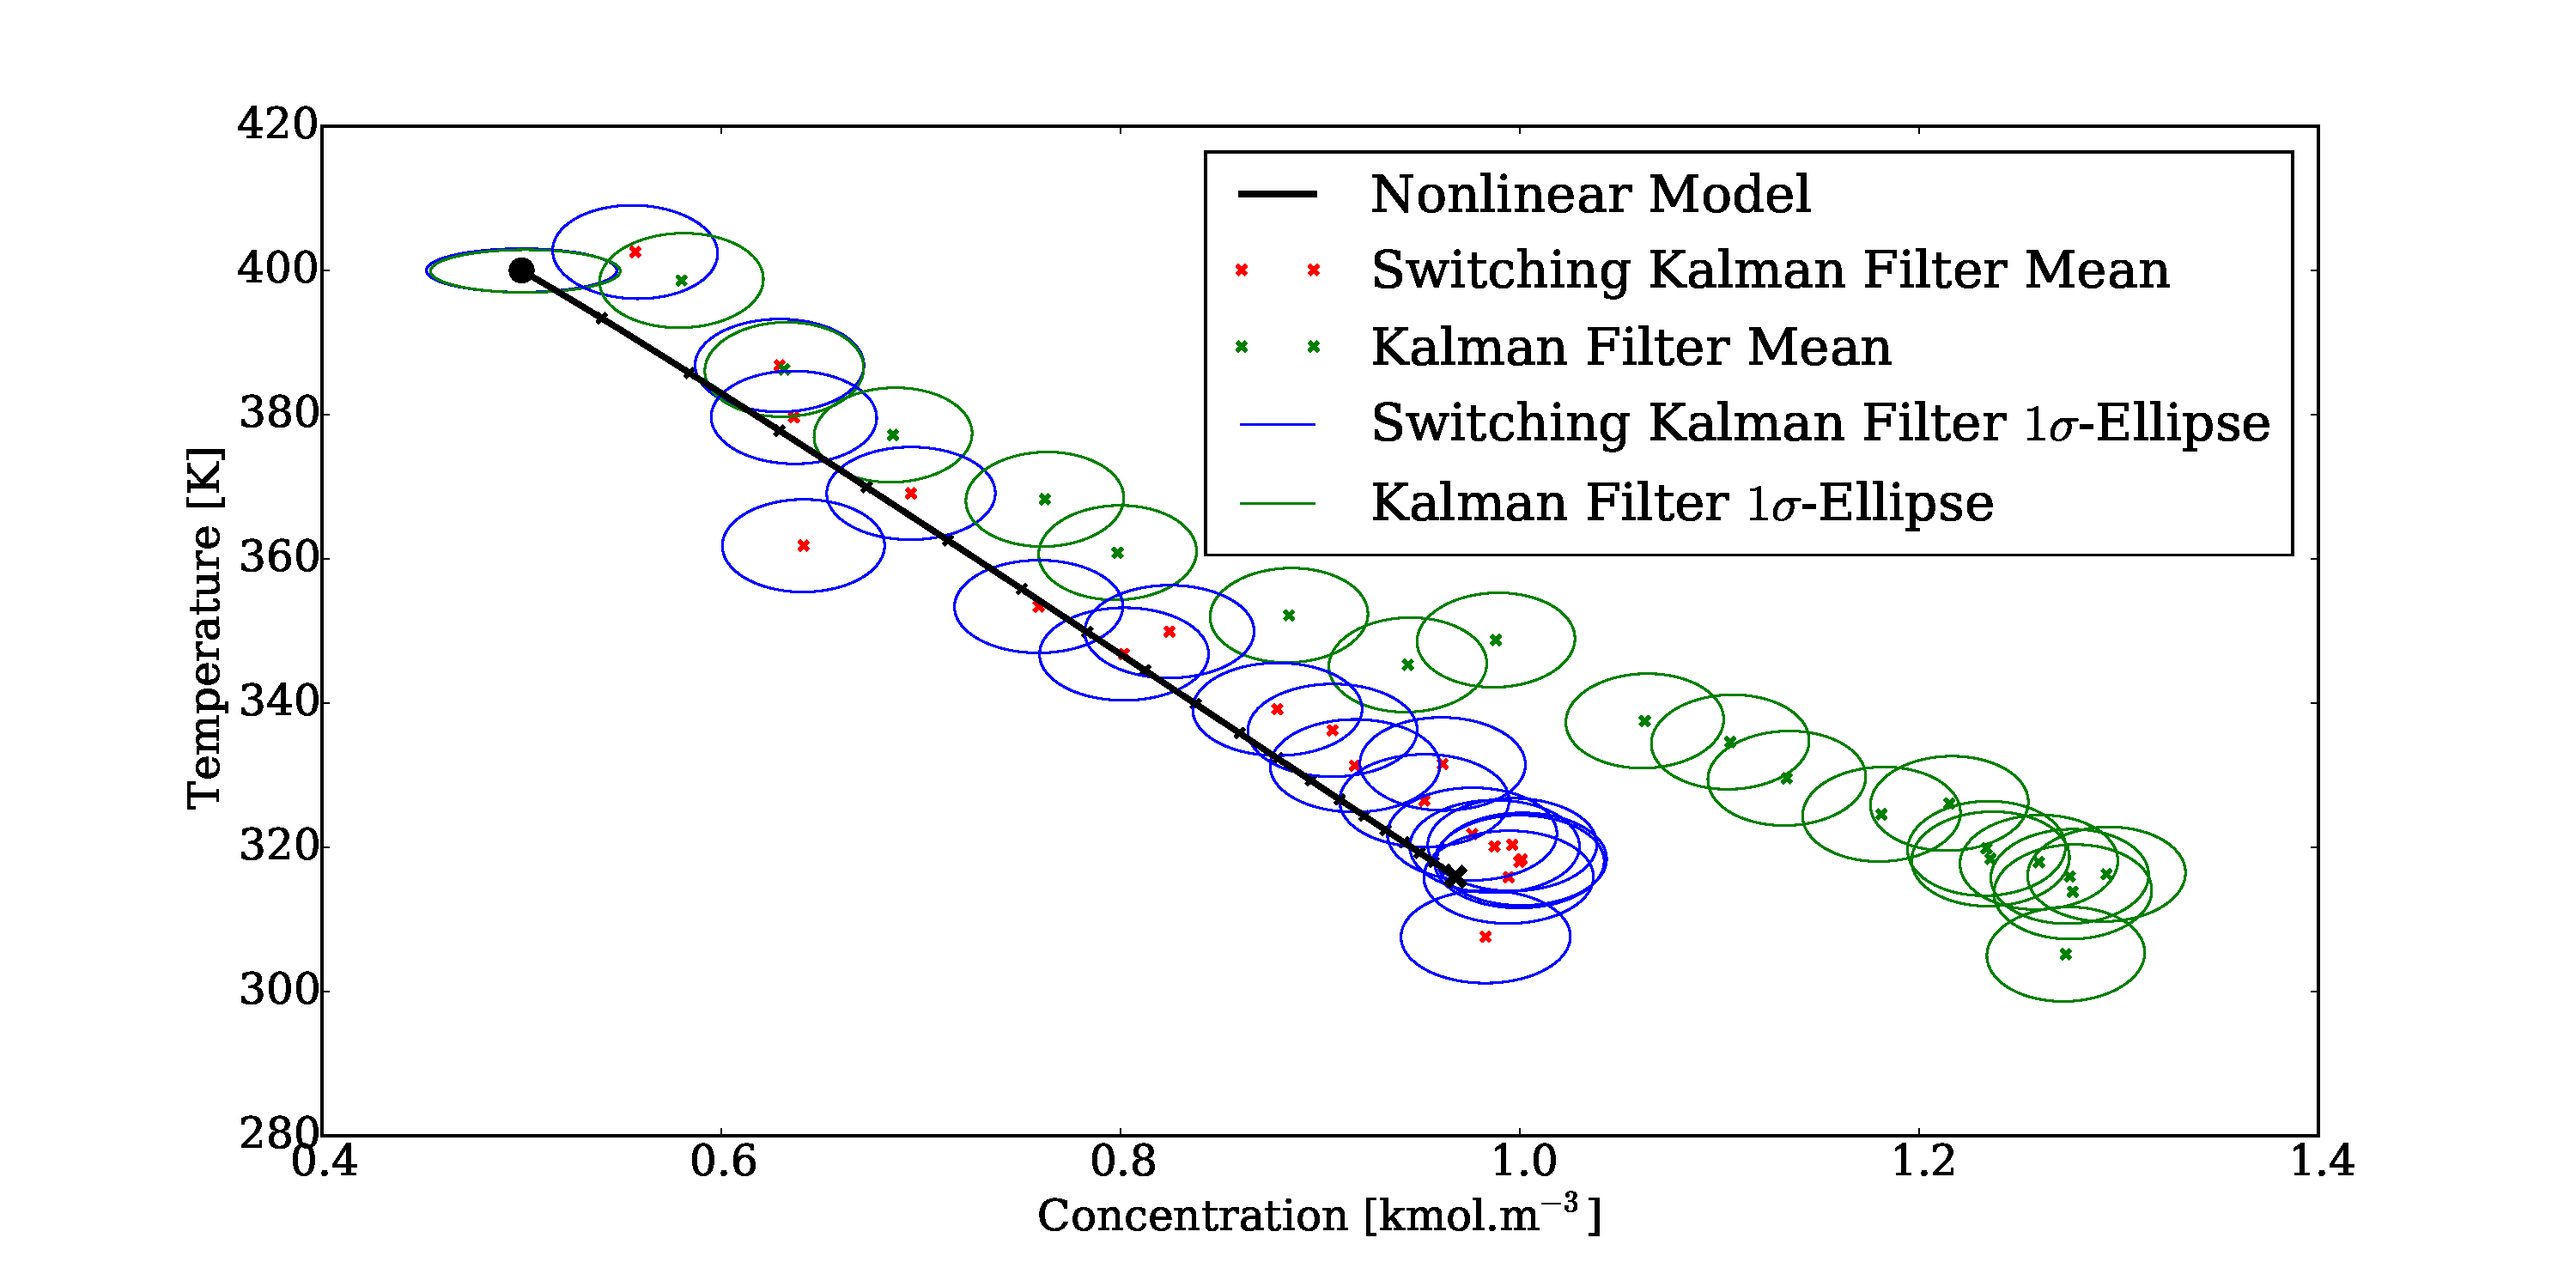
\includegraphics[scale=0.3]{skf_s7_p_m2_b.pdf}
\caption{State space evolution of the Switching Kalman Filter and the standard Kalman filter which only uses one linear model.}
\label{fig_7mod_p_m2_b}
\end{figure}
The primary benefit of the Switching Kalman Filter is its ability to choose which models to use based on the observations. Although the technique is significantly more computationally intensive it is beneficial in situations where a single linear model does not adequately describe the system. 